\section{About the EROS training set}

We use a training data set provided by \citet{kim2014} which contains labels (main and sub--classes) and lightcurves for $32655$ sources in the Large Magellanic Cloud (LMC). The lightcurves were recorded by the Expérience pour la Recherche d’Objets Sombres (EROS) project, a wide--field survey. A thorough description of the compilation process is available in \citet{kim2014}, however, here is a list of the main steps:

\begin{enumerate}
\item Compile known periodoic variables in the LMC from the OGLE and MACHO surveys
\item Add $982$ blue variables (BVs) from the MACHO database
\item Add 565 quasi--stellar objects (QSOs)
\item 
\end{enumerate}

% Number of sources in the data set
% Not a standard astronomical B and R bands

\section{Feature Extraction}

We extract a variety of features characterizing the variability of the source. A lot of them are standard statistical features, but some are more sophisticated, trying to incorporate a model of the underlying physics. In the following, $N$ will be the number of data points in the light curve, $(t_i, m_i)$ the $i^{\text{th}}$ data point in the light curve. Some of the features are extracted from the recorded lightcurve, as well as from the phase--folded lightcurve ($P_{\text{LS}}$). We label the latter with a superscript $\phi$, \eg $\mu^\phi, \sigma^\phi$ and so forth\footnote{Note that this does not necessarily mean that \emph{all} features based on a phase--folded lightcurve are labelled this way.}.

\begin{enumerate}
%\setlength{\itemsep}{5pt}
%\setlength{\parskip}{0pt}
%\setlength{\parsep}{0pt}
%\setlength{\abovedisplayskip}{.5em}
%\setlength{\belowdisplayskip}{.5em}

\litem{$\mu, \mu^\phi$ (Mean of magnitude)} The arithmetic mean of the magnitude, given by
\begin{equation}\mu = \frac{1}{N} \sum\limits_{i=1}^{N} m_i.\end{equation}

\litem{$\sigma, \sigma^\phi$ (Standard deviation of magnitude)} The standard deviation of the magnitude, given by
\begin{equation}\sigma = \sqrt{\frac{1}{N-1} \sum_{i=1}^N (m_i - \mu)^2}.\end{equation}

\litem{$Q_{50}, Q_{50}^\phi$ (Median of magnitude)} The median of the magnitude, given by
\begin{equation}Q_{50} = \tilde m_{\lfloor\frac{N+1}{2}\rfloor},\end{equation}
where $\tilde m$ is the sorted list of magnitude with legth $N$.

\litem{$\bar \mu, \bar \mu^\phi$ (Weighted mean of magnitude)} The weighted arithmetic mean of the magnitude, given by
\begin{equation}\bar \mu = \big(\sum\limits_{i=1}^{N} w_i m_i\big) \; / \; \big(\sum\limits_{i=1}^{N} w_i\big),\end{equation}
with weights $w_i$ inversely proportional to the measurement uncertainty, \ie $w_i = \sigma_i^{-1}$ with $\sigma_i > 0 \; \forall i$.

\litem{$\bar \sigma, \bar \sigma^\phi$ (Weighted standard deviation of magnitude)} The weighted standard deviation of the magnitude, given by
\begin{equation}\bar \sigma = \sqrt{\frac{1}{(N-1) \sum\limits_{i=1}^{N} w_i} \sum_{i=1}^N w_i \, ( m_i - \bar \mu)^2}.\end{equation}

\litem{$\gamma_1, \gamma_1^\phi$ (Skewness)} The skewness of the magnitude, given by
\begin{equation}\gamma_1 = \frac{N}{(N-1)(N-2)} \sum\limits_{i=1}^N \big( \frac{m_i - \mu}{\sigma} \big)^3.\end{equation}

\litem{$\gamma_2, \gamma_2^\phi$ (Kurtosis)} The kurtosis of the magnitude, given by
\begin{equation}\gamma_2 = \frac{N(N+1)}{(N-1)(N-2)(N-3)} \sum\limits_{i=1}^N \big( \frac{m_i - \mu}{\sigma} \big)^4 - 3 \, \frac{(N-1)^2}{(N-2)(N-3)}.\end{equation}

\litem{$Q_{25}, Q_{25}^\phi$ ($25^\text{th}$ percentile)} The $25^\text{th}$ percentile of the magnitude, given by
\begin{equation}Q_{25} = \cdots.\end{equation}

\litem{$Q_{75}, Q_{75}^\phi$ ($75^\text{th}$ percentile)} The $75^\text{th}$ percentile of the magnitude, given by
\begin{equation}Q_{75} = \cdots.\end{equation}

\litem{$\text{IQR}, \text{IQR}^\phi$ (Interquartile range)} The interquartile range of the magnitude, given by
\begin{equation}\text{IQR} = Q_{75} -Q_{25}.\end{equation}

\litem{$T_{\text{LS}}$ (Lomb--Scargle period)} The maximum--likelihood period according to the Lomb--Scargle periodogram, given by
\begin{equation}P_{\text{LS}} = \frac{1}{2 \sigma_y^2} \Bigg\{ \frac{\big[\sum\limits_{i=1}^k (y_i - \mu_y) \cos(\omega(t_i - \tau))\big]^2}{\sum\limits_{i=1}^k \cos^2(\omega(t_i - \tau))} + \frac{\big[\sum\limits_{i=1}^k (y_i - \mu_y) \sin(\omega(t_i - \tau))\big]^2}{\sum\limits_{i=1}^k \sin^2(\omega(t_i - \tau))}\Bigg\}\end{equation}

\litem{$\text{FAP}_{\text{LS}}$ (False--Alarm probability for Lomb--Scargle)} The false--alarm probability (FAP) for the Lomb--Scargle algorithm, given by
\begin{equation}\text{FAP}_{\text{LS}}(x) = 1 - (1 - \euler^{-x})^M.\end{equation}

\litem{$\text{SNR}, \text{SNR}^\phi$ (Signal--to--noise ratio)} The signal--to--noise ratio, given by
\begin{equation}\text{SNR} = \frac{\mu}{\sigma}.\end{equation}

\litem{$S, S^\phi$ (Shannon entropy)} The Shannon entropy \citep{shannon1949} of the signal, given by
\begin{equation}S = -\sum\limits_{i=1}^N m_i \ln(m_i).\end{equation}

\litem{$\eta, \eta^\phi$ (Eta--feature)} The $\eta$ feature as proposed by \citet{vonneumann1941}, given by
\begin{equation}\eta = \frac{1}{\sigma^2 (N-1)} \sum\limits_{i=1}^{N-1} (m_{i+1} - m_{i})^2.\end{equation}

\litem{$\eta_e, \eta_e^\phi$ (Eta--feature)} $\eta_e$ is an enhancement of the $\eta$-feature by \citet{kim2014}, that accounts for unequal sampling, given by
\begin{equation}\eta_e = (\frac{1}{N-1}\sum_{i=1}^{N-1} w_i) (t_{N-1} - t_1)^2 \big( \sum\limits_{i=1}^{N-1} w_i (m_{i+1} + m_i)^2 \big) \, / \, \big( \sigma^2 \sum\limits_{i=1}^{N-1} w_i \big),\end{equation}
where the weights are given by $w_i = (t_{i+1} - t_i)^{-2}$.

\litem{$\cdots$ (Half--magnitude--amplitude ratio)} The ratio of higher \resp lower amplitudes than average, given by
\begin{equation}\cdots = \sqrt{ \Big(\sum\limits_{l=1}^N \big( \alpha^{>}_l - \mu \big)^2\Big) \, / \, \Big(\sum\limits_{m=1}^N \big( \alpha^{<}_m - \mu \big)^2\Big)},\end{equation}
where $\alpha^{>}, \alpha^{<}$ are magnitudes higher resp. lower than $\mu$.

\litem{$\text{MAD}_{\mu}, \text{MAD}_{\mu}^\phi$ (Mean absolute deviation)} The mean absolute deviation of the magnitude, given by
\begin{equation}\text{MAD}_{\mu} = \frac{1}{N} \sum\limits_{i=1}^{N} | m_i - \mu |.,\end{equation}
which is essentially the average distance between each of the data points and the mean.

\litem{$\text{MAD}_{Q_{50}}, \text{MAD}_{Q_{50}}^\phi$ (Median absolute deviation)} The median absolute deviation of the magnitude, given by
\begin{equation}\text{MAD}_{Q_{50}} = .\end{equation}

\litem{$W_{\text{SW}}, p_{\text{SW}}$ (Shapiro--Wilk statistics)} The Shapiro--Wilk test \citep{shapiro1965} is used to test the null hypothesis that the data was drawn from a normal distribution. We the features
\begin{equation}W_{\text{SW}} = \big(\sum\limits_{i=1}^n \lambda_i m_{(i)}\big)^2 \, / \, \big(\sum\limits_{i=1}^n (m_i - \mu)^2\big).\end{equation}
as features, where $\lambda_i$ are constants derived from means, and variances of a normally distributed sample of the same size, $m_{(i)}$ is the $i^\text{th}$ smallest value in $m$, and $p_{\text{SW}}$ is the $p$-value for the hypothesis test.

\litem{$\text{SF}$ (Structure function features)} We extract $A, \sigma_A, \gamma, \sigma_\gamma$ from the structure function power--law fit, $A \big(\frac{\Delta t}{1 \, \mathrm{yr}}\big)^\gamma$, where the structure function is defined as
\begin{equation}\text{SF}(\Delta t) = \big\langle \sqrt{\frac{\pi}{2}} \big| \Delta m_{ij}  \big| - \sqrt{\sigma_{m_i}^2 + \sigma_{m_j}^2} \big\rangle_{\Delta t},\end{equation}
where $\langle \cdot \rangle$ is the mean of the data points within the bin $\Delta t$.

\litem{$\mathcal{F}$ (Fourier features)} We fit standard fourier series with five terms to the phase--folded lightcurve.
\begin{equation}\mathcal{F}(t) = \frac{A_0}{2} + \sum_{k=1}^{\infty} ( A_k \cos(2 \pi k t) + B_k \sin(2 \pi k t) ).\end{equation}
From this we the extract amplitude and phase features $A_0$, $A_i = \sqrt{a_i^2 + b_i^2}$ and $\varphi_i = \arctan(\frac{b_i}{a_i})$ features for $i = 1, \ldots, 5$.

\litem{$T_{\text{CE}_1}, T_{\text{CE}_2}, T_{\text{CE}_3}$ (CE periods)} We add three candidate periods with the lowest conditional entropy according to the CE periodogram, given by
\begin{equation}P_{\text{CE}} = \cdots.\end{equation}
Furthermore, we also add the CE scores, $\text{CE}_1, \text{CE}_2, \text{CE}_3$, for each of the periods as features.

\litem{$\delta_{\text{CE}_1}, \delta_{\text{CE}_2}$ ($\delta_{\text{CE}}$ features)} We add two more features comparing $T_{\text{LS}}$ and $T_{\text{CE}_1}$, which we define as
\begin{equation}\delta_{\text{CE}_1} = T_{\text{LS}} - T_{\text{CE}_1}, \, \delta_{\text{CE}_2} = \frac{\delta_{\text{CE}_1}}{T_{\text{LS}}}.\end{equation}

\litem{$\Delta_{Q_{10}}^\phi, \Delta_{Q_{90}}^\phi$ (Slope percentile features)} The $10^\text{th}$ and $90^\text{th}$ percentile of the slope, given by
\begin{equation}\Delta = \frac{(t_{i+1} - t_i)}{(m_{i+1} - m_i)}.\end{equation}

\litem{$\Sigma, \Sigma^\phi$ (Cumulative sum)} The range $\max(S) - \min(S)$ of the cumulative sum \citep{ellaway1978} of $S_k$, given by
\begin{equation}S_k = \frac{1}{\sigma N} \sum\limits_{i=1}^k (m_i - \mu) .\end{equation}

\litem{$K$ (Stetson $K$)} The Stetson K index \citep{stetson1996}, given by
\begin{equation}K = \frac{1}{\sqrt{N}} \big( \sum\limits_{i=1}^N |\delta_i| \big) \, / \, \big( \sqrt{\sum\limits_{i=1}^N \delta_i^2} \big) \text{ with } \delta_i = \sqrt{\frac{N}{N-1}} \frac{m_i - \mu}{\sigma_i}.\end{equation}

% Proper citing of all equations

\end{enumerate}

This leads to a total of $\cdots$ features in $\cdots$ bands.

\begin{figure}[h]
	\centering
	\begin{subfigure}[t]{0.49\textwidth}
		\centering
		\caption{$T_{\text{LS}}$ ($B_E$) vs. $\eta^\phi$ ($B_E$)}
		\label{fig:2a}
		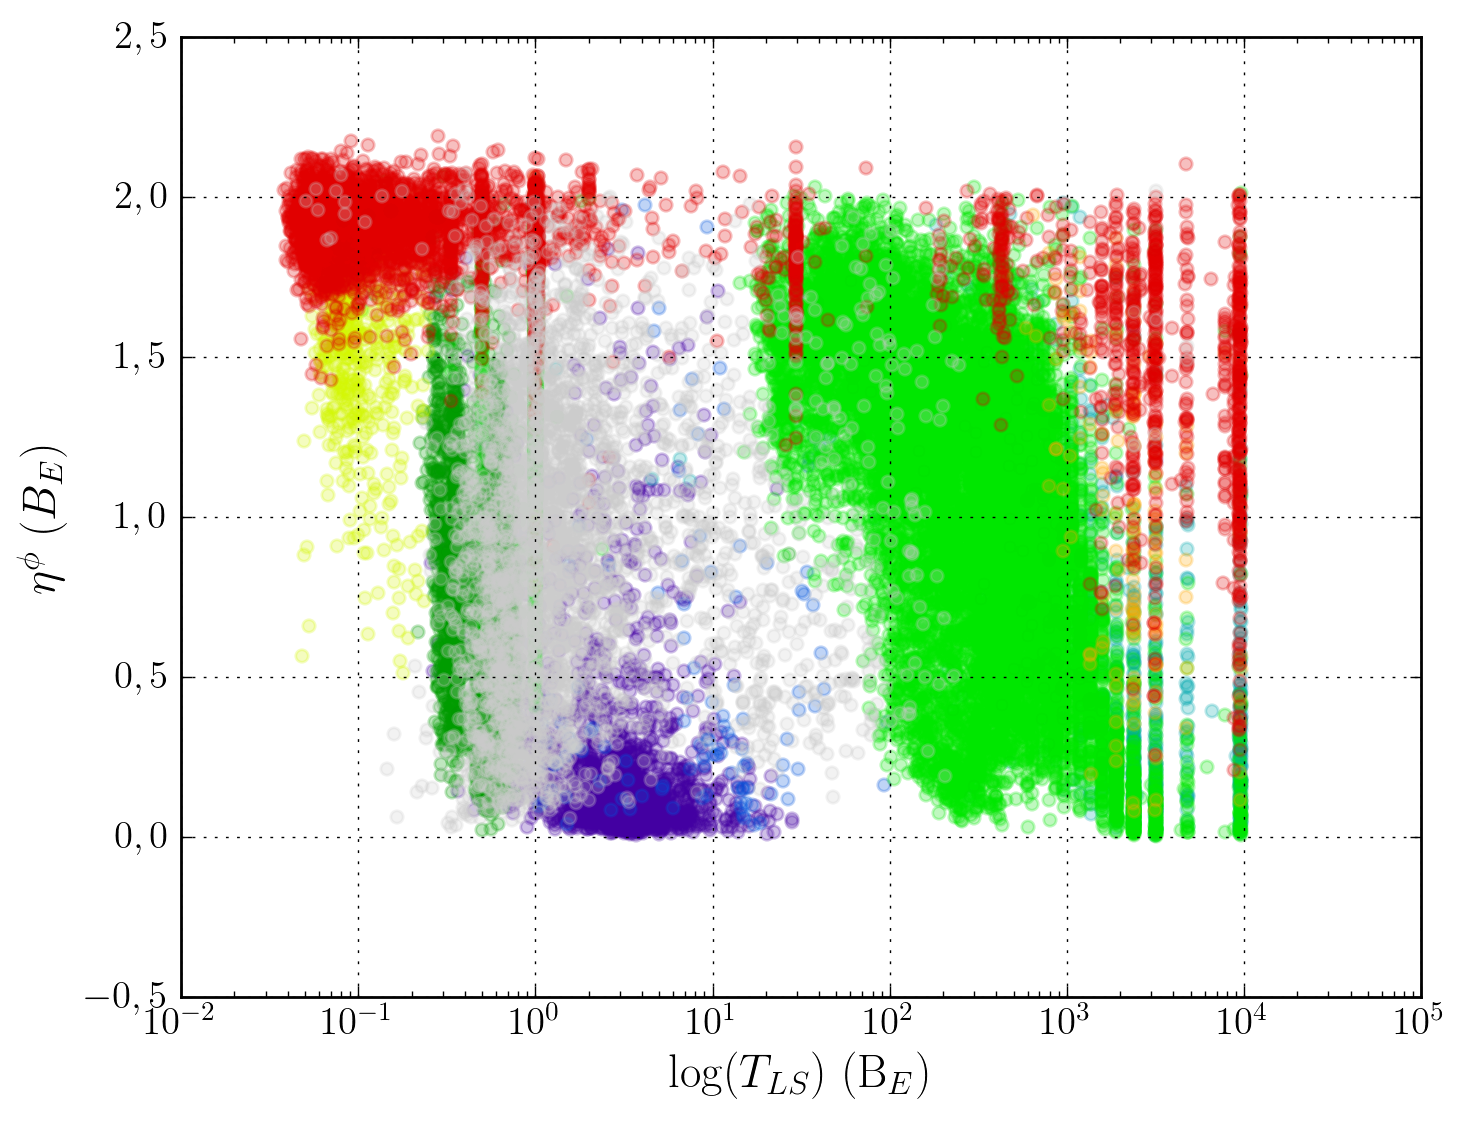
\includegraphics[width=\textwidth]{figures/scatterplots/B-ls-period-B-phase-eta.png}				
	\end{subfigure}
	\begin{subfigure}[t]{0.49\textwidth}
		\centering
		\caption{$\eta$ ($B_E$) vs. $\Sigma^\phi$ ($B_E$)}
		\label{fig:2b}
		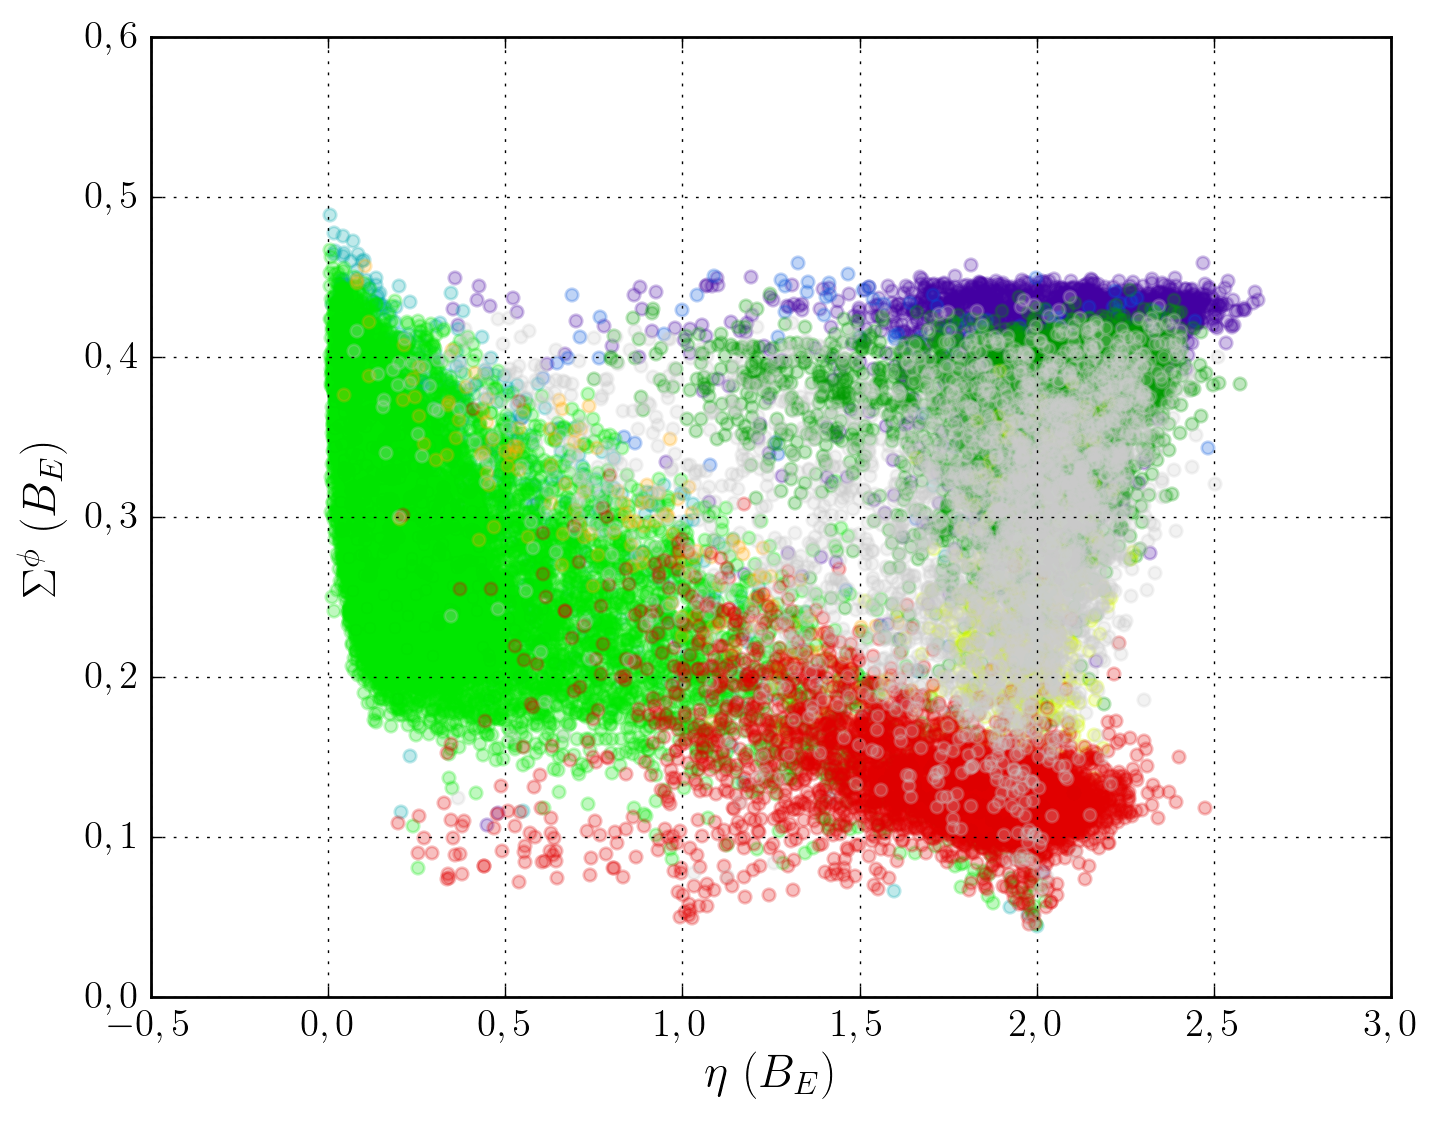
\includegraphics[width=\textwidth]{figures/scatterplots/B-eta-B-phase-cs.png}		
	\end{subfigure}
	\begin{subfigure}[t]{0.49\textwidth}
		\centering
		\caption{$\eta$ ($B_E$) vs. $\log(\eta_e)$ ($B_E$)}
		\label{fig:2c}
		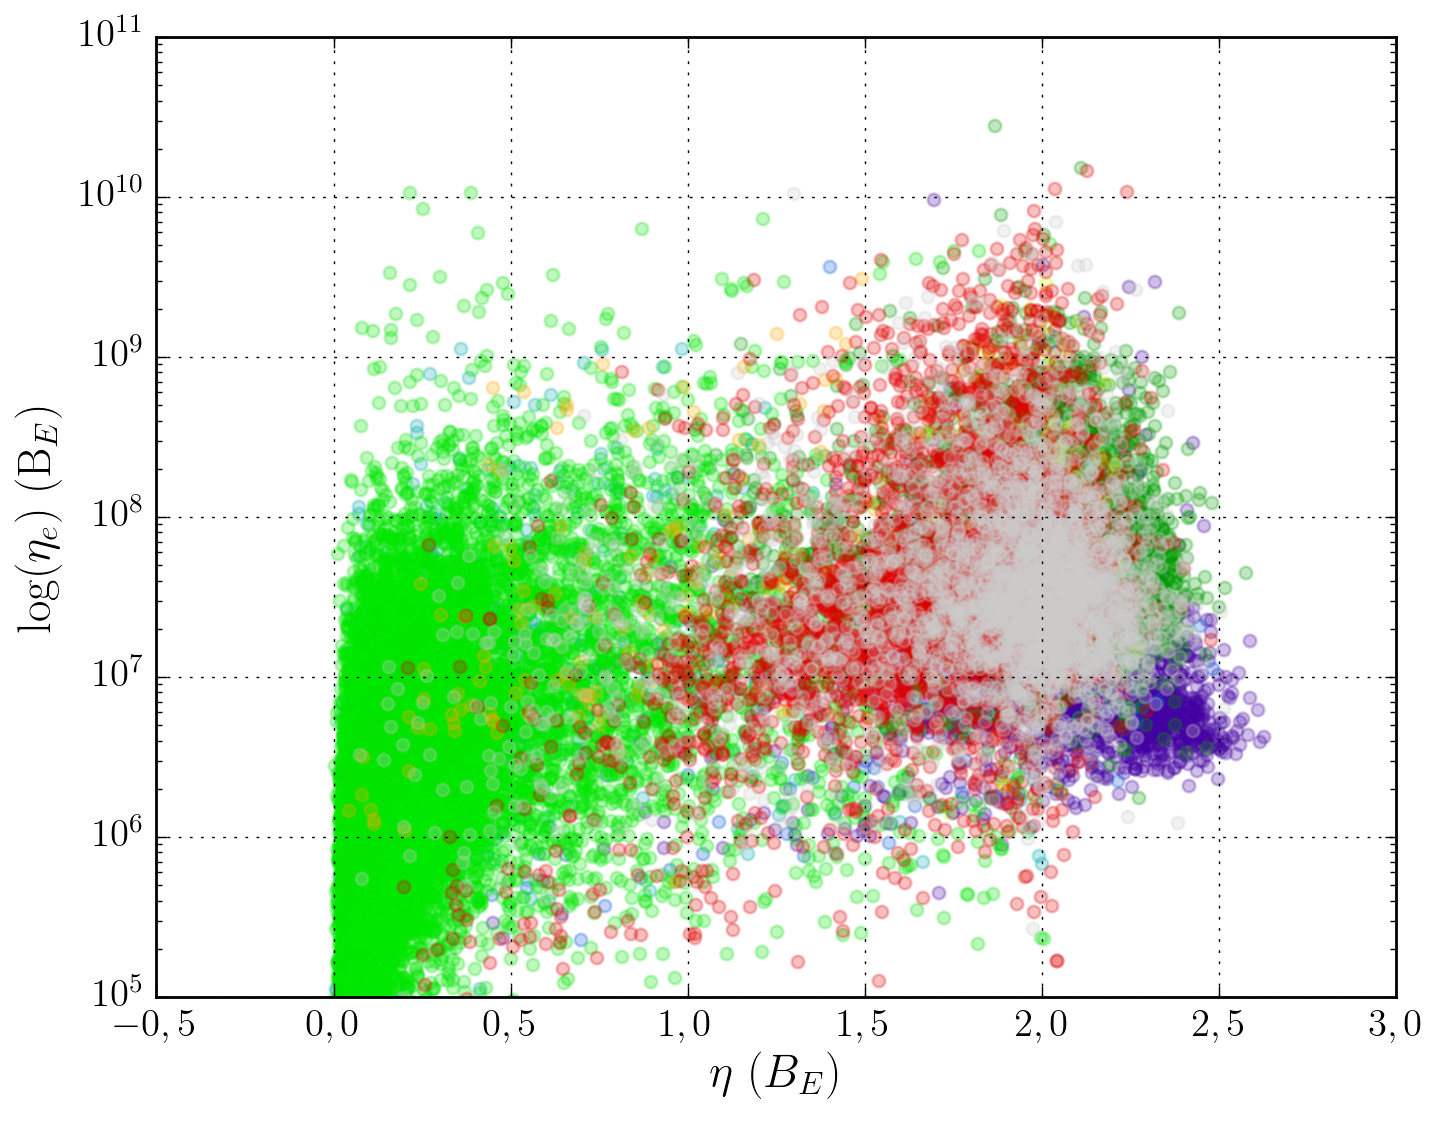
\includegraphics[width=\textwidth]{figures/scatterplots/B-eta-B-eta-e.png}		
	\end{subfigure}
	\begin{subfigure}[t]{0.49\textwidth}
		\centering
		\caption{$\mu$ ($B_E$) vs. $\mu$ ($R_E - B_E$)}
		\label{fig:2d}
		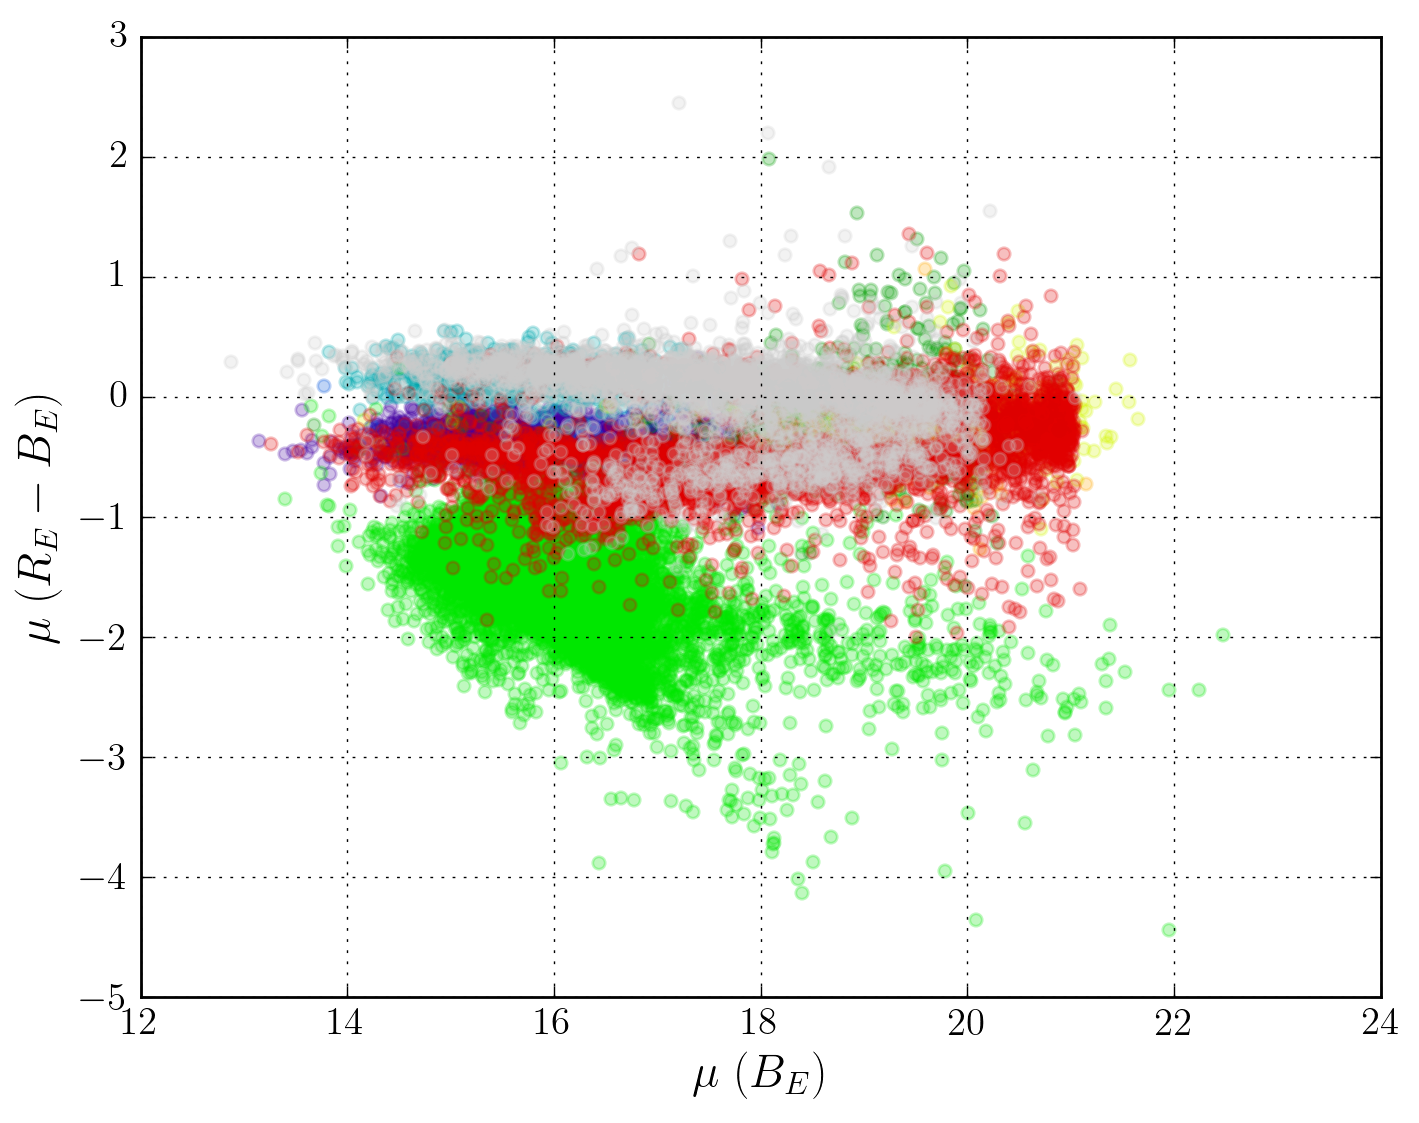
\includegraphics[width=\textwidth]{figures/scatterplots/B-mean-R-B-mean.png}		
	\end{subfigure}
	\begin{subfigure}[t]{0.49\textwidth}
		\centering
		\caption{$\Sigma^\phi$ ($B_E$) vs. $\log(\text{IQR})$ ($R_E - B_E$)}
		\label{fig:2e}
		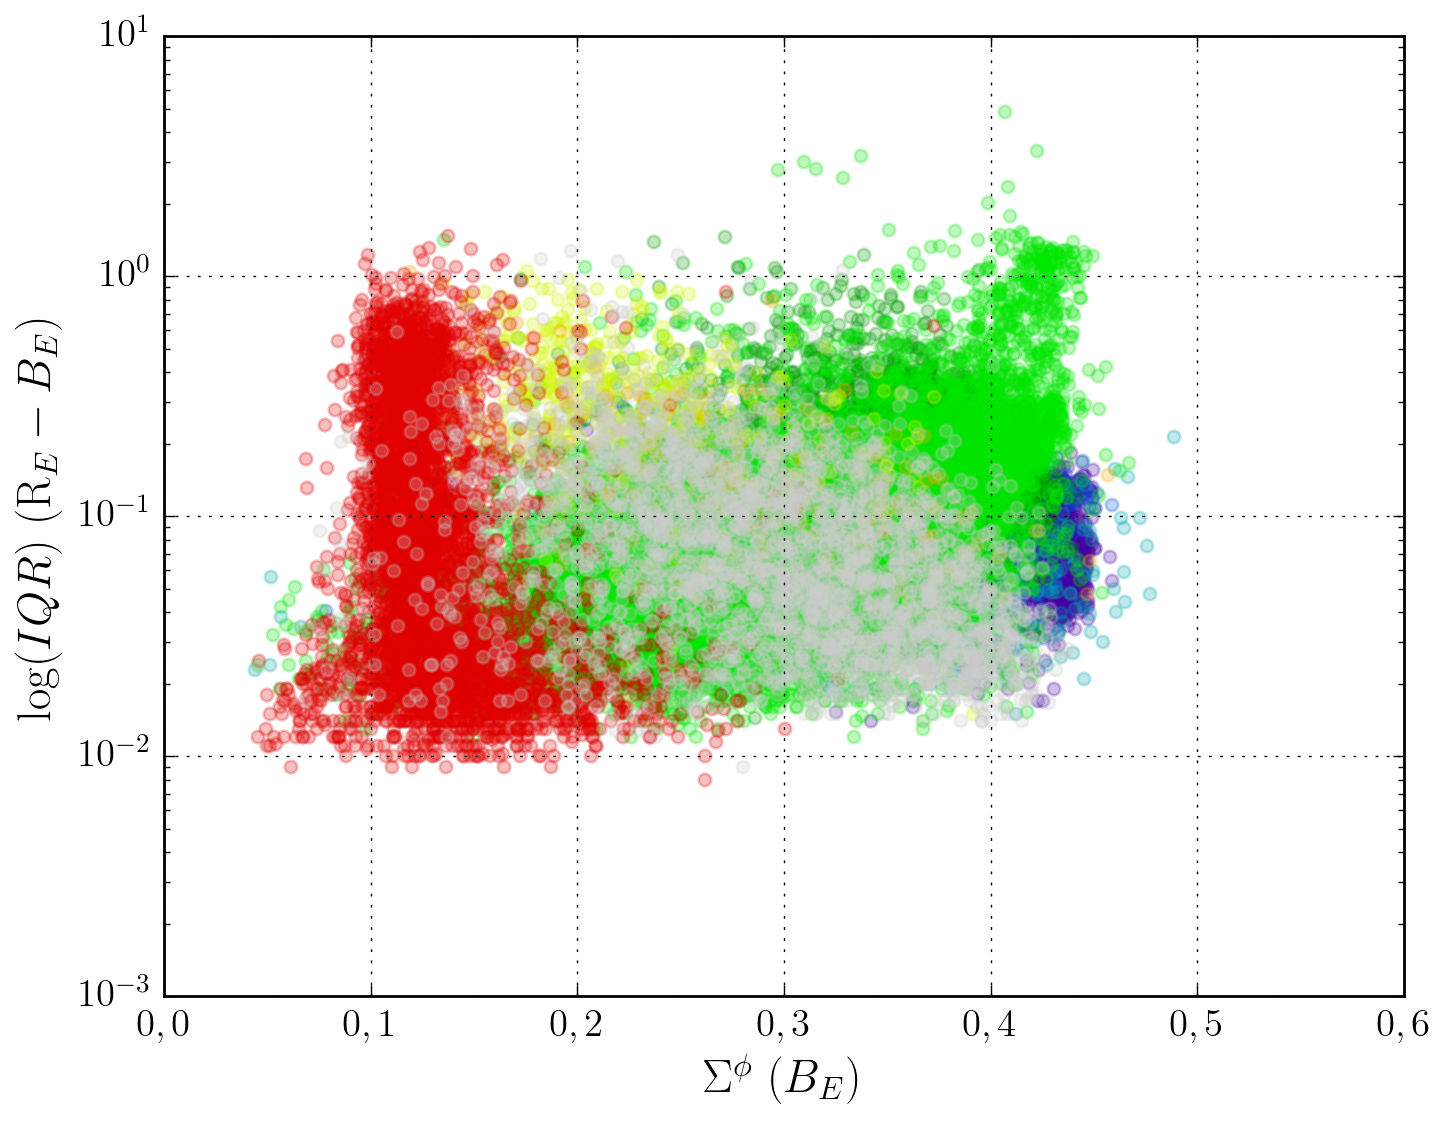
\includegraphics[width=\textwidth]{figures/scatterplots/B-phase-cs-R-B-IQR.png}		
	\end{subfigure}
	\begin{subfigure}[t]{0.49\textwidth}
		\centering
		\caption{$\log(T_{\text{LS}})$ ($R_E$) vs. $Q_{25}^\phi$ ($R_E$)}
		\label{fig:2f}
		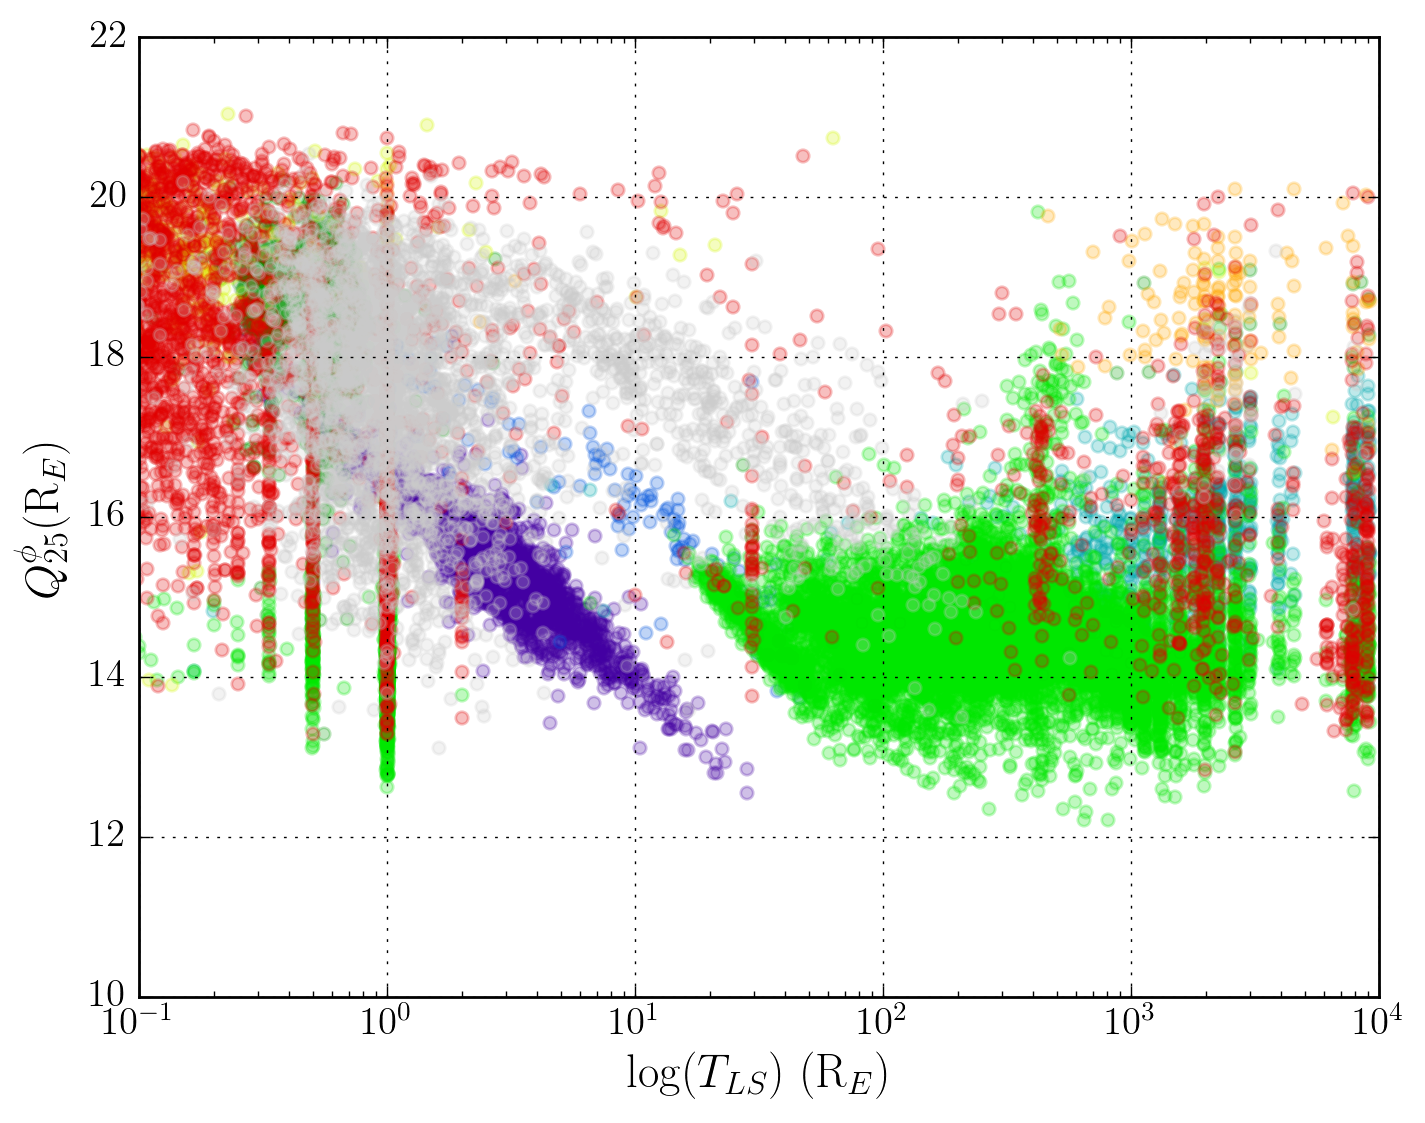
\includegraphics[width=\textwidth]{figures/scatterplots/R-ls-period-R-phase-q25.png}		
	\end{subfigure}
	\caption{This figure shows different scatterplots. $\cdots$\\\colorlegend}
	\label{fig:2}
\end{figure}

% State that feature are highly correlated
% Show histogram of some features.
% Show some scatterplots
% More about period finding

\section{Performance of the Support Vector Machine}

The first classifier we try is the Support Vector Machine (SVM) with the RBF kernel $\kernel_{\text{RBF}}$. We optimize the models hyperparameters $C$ and $\gamma$ for the average, weighted $F_1$-score by performing a $5$-fold cross--validation on subsequently finer grids. The results are visualized in figure \ref{fig:gridsearch-svm-superclasses}.

\begin{figure}[h]
	\centering
	\begin{subfigure}[t]{0.49\textwidth}
		\centering
		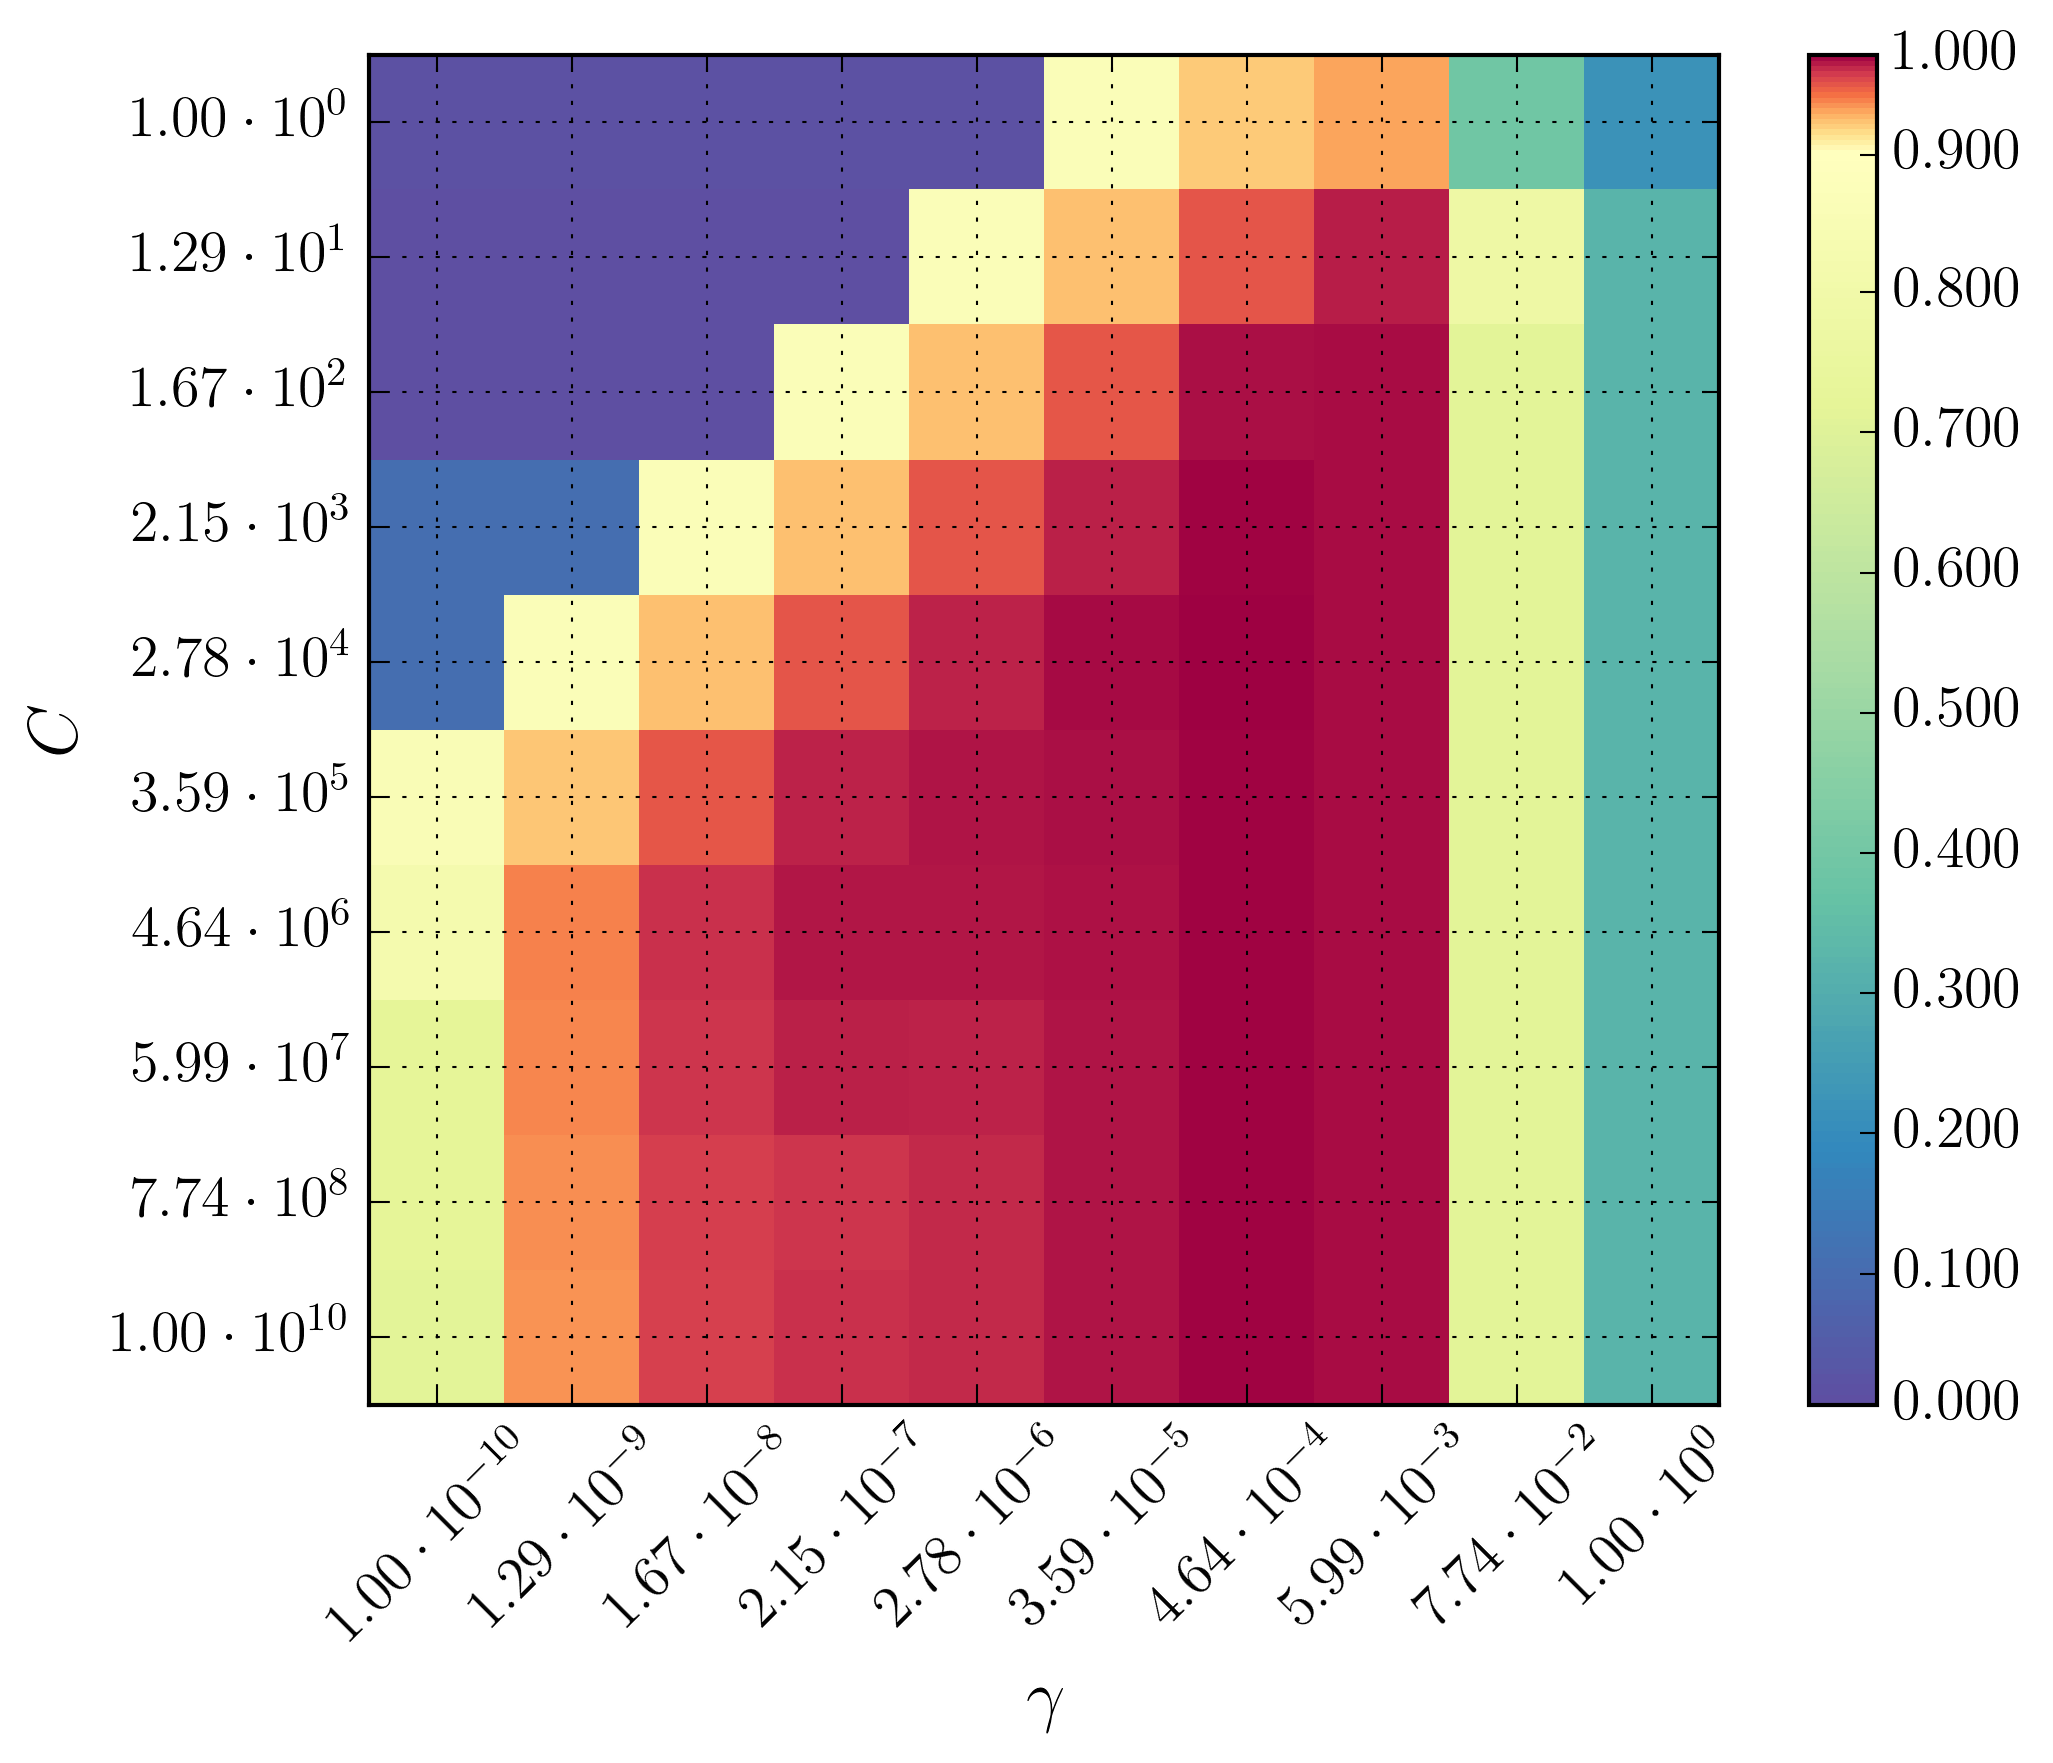
\includegraphics[width=\textwidth]{figures/gridsearch/svm/superclasses/svm-superclasses-01.png}				
	\end{subfigure}
	\begin{subfigure}[t]{0.49\textwidth}
		\centering
		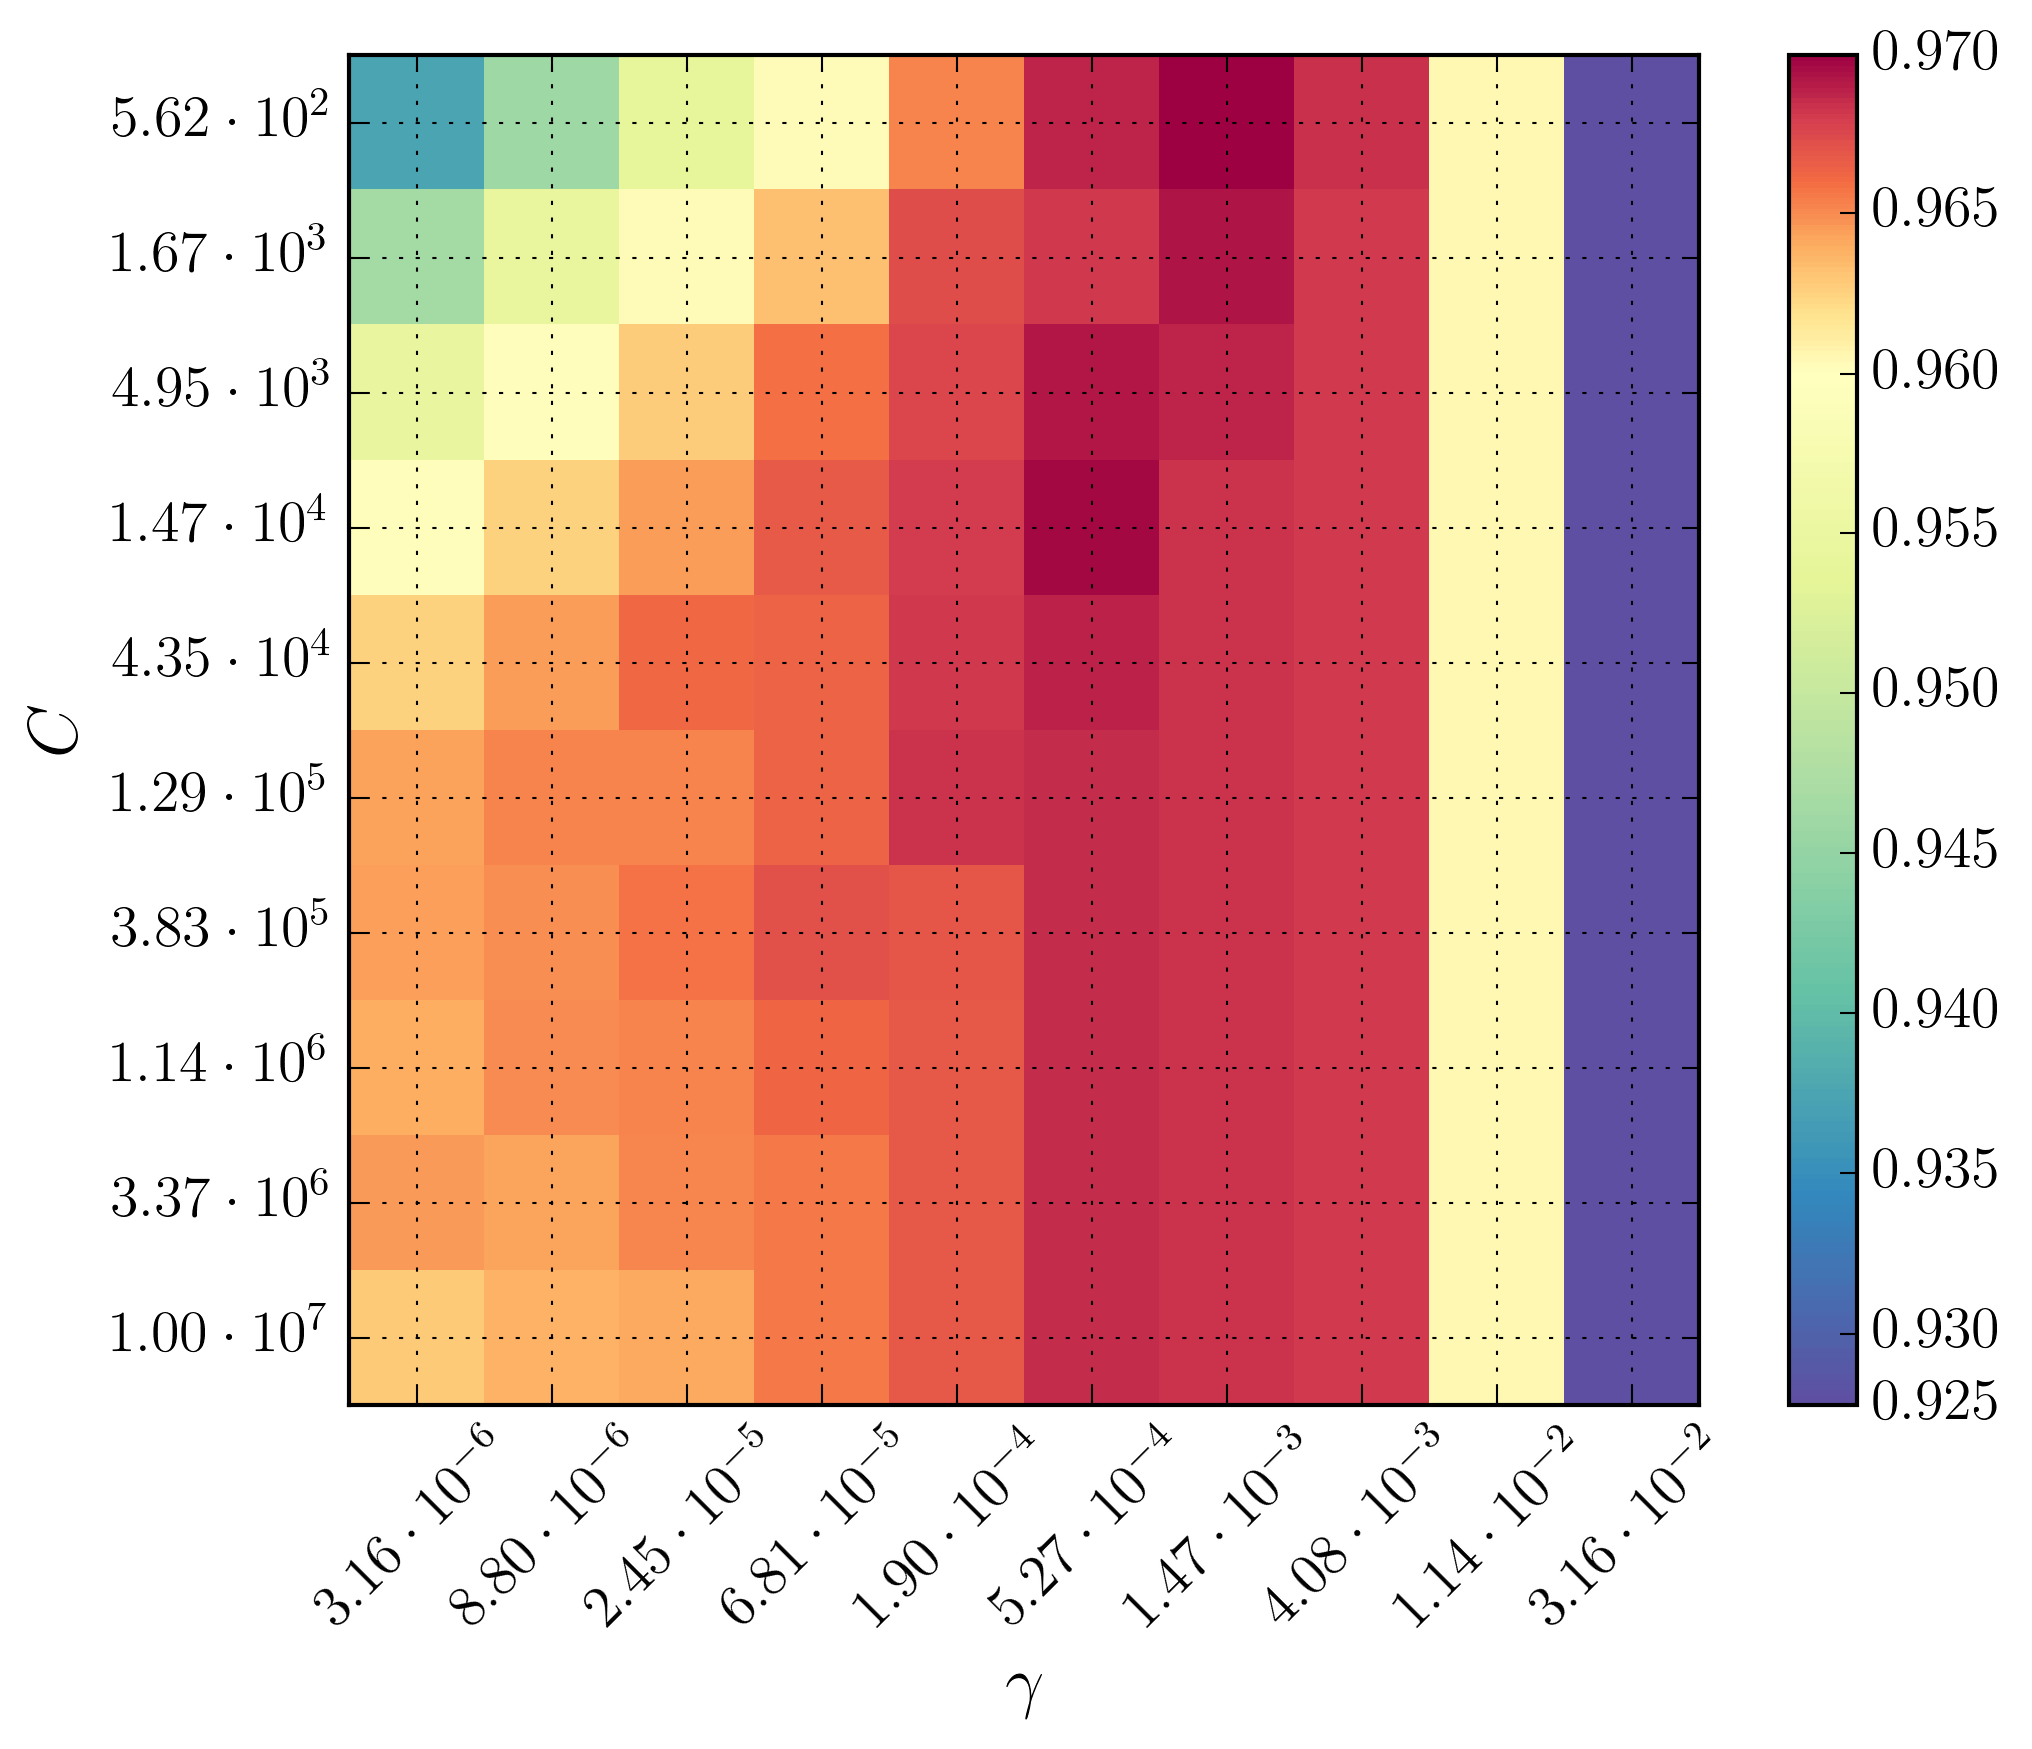
\includegraphics[width=\textwidth]{figures/gridsearch/svm/superclasses/svm-superclasses-02.png}		
	\end{subfigure}
	\begin{subfigure}[t]{0.49\textwidth}
		\centering
		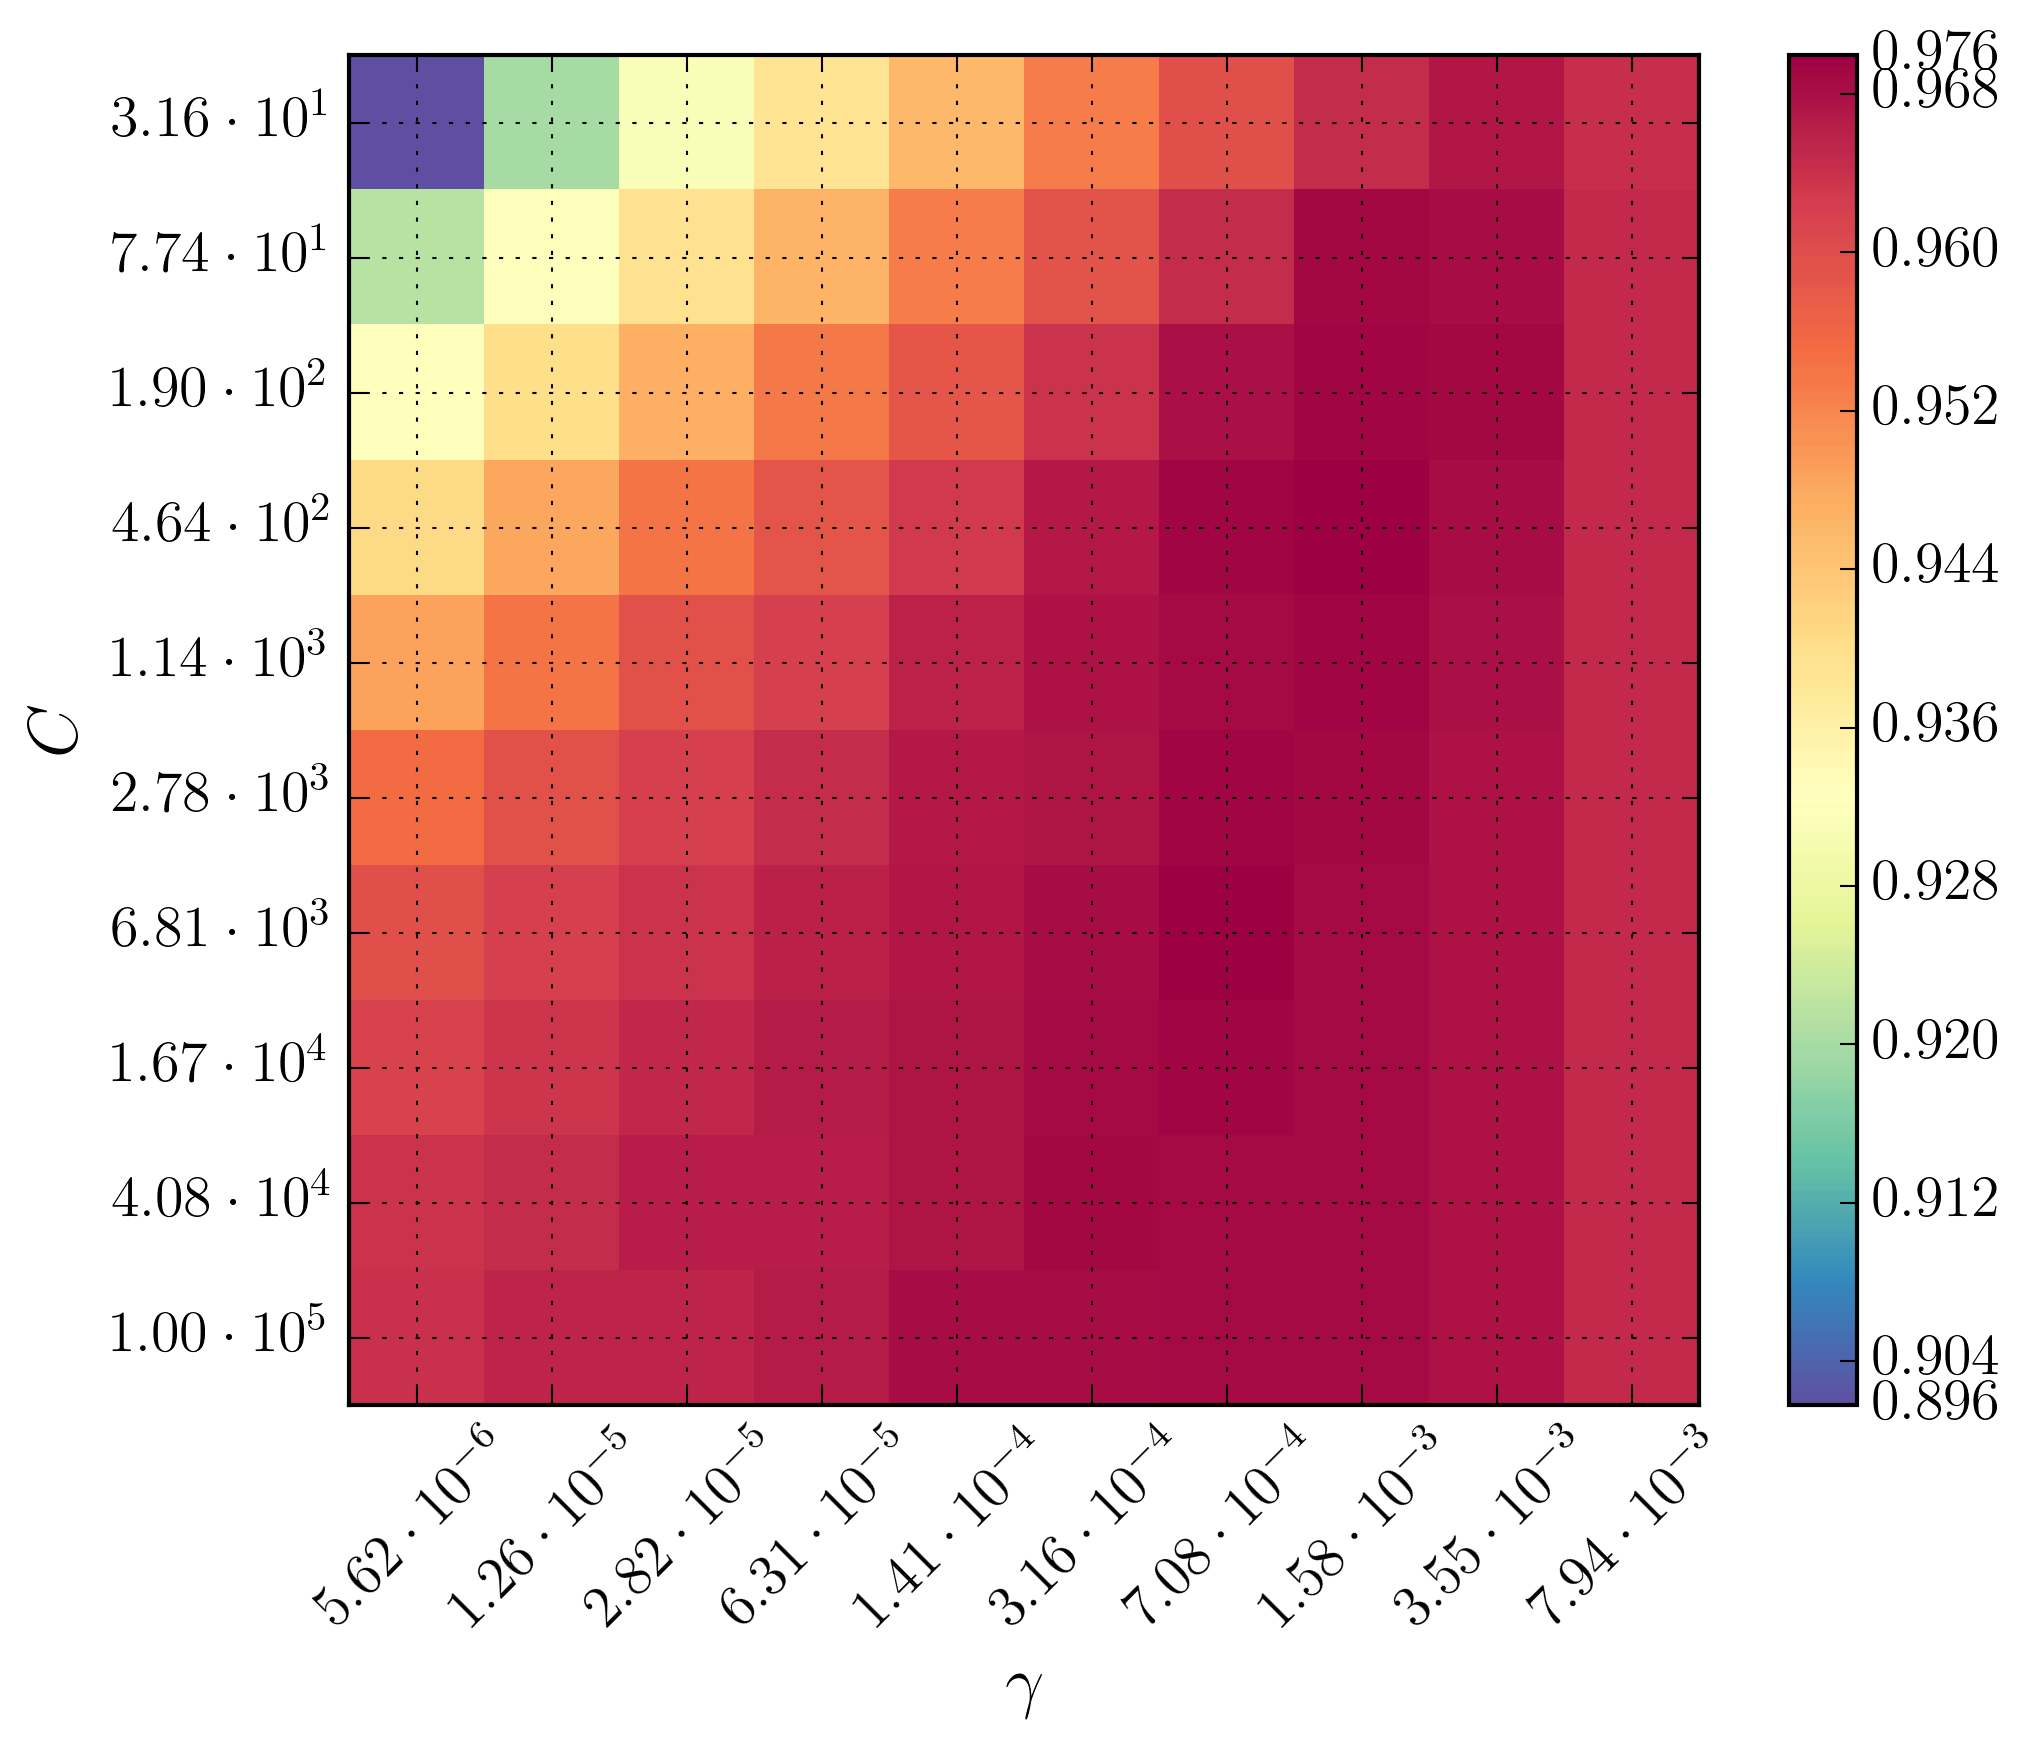
\includegraphics[width=\textwidth]{figures/gridsearch/svm/superclasses/svm-superclasses-03.png}				
	\end{subfigure}
	\begin{subfigure}[t]{0.49\textwidth}
		\centering
		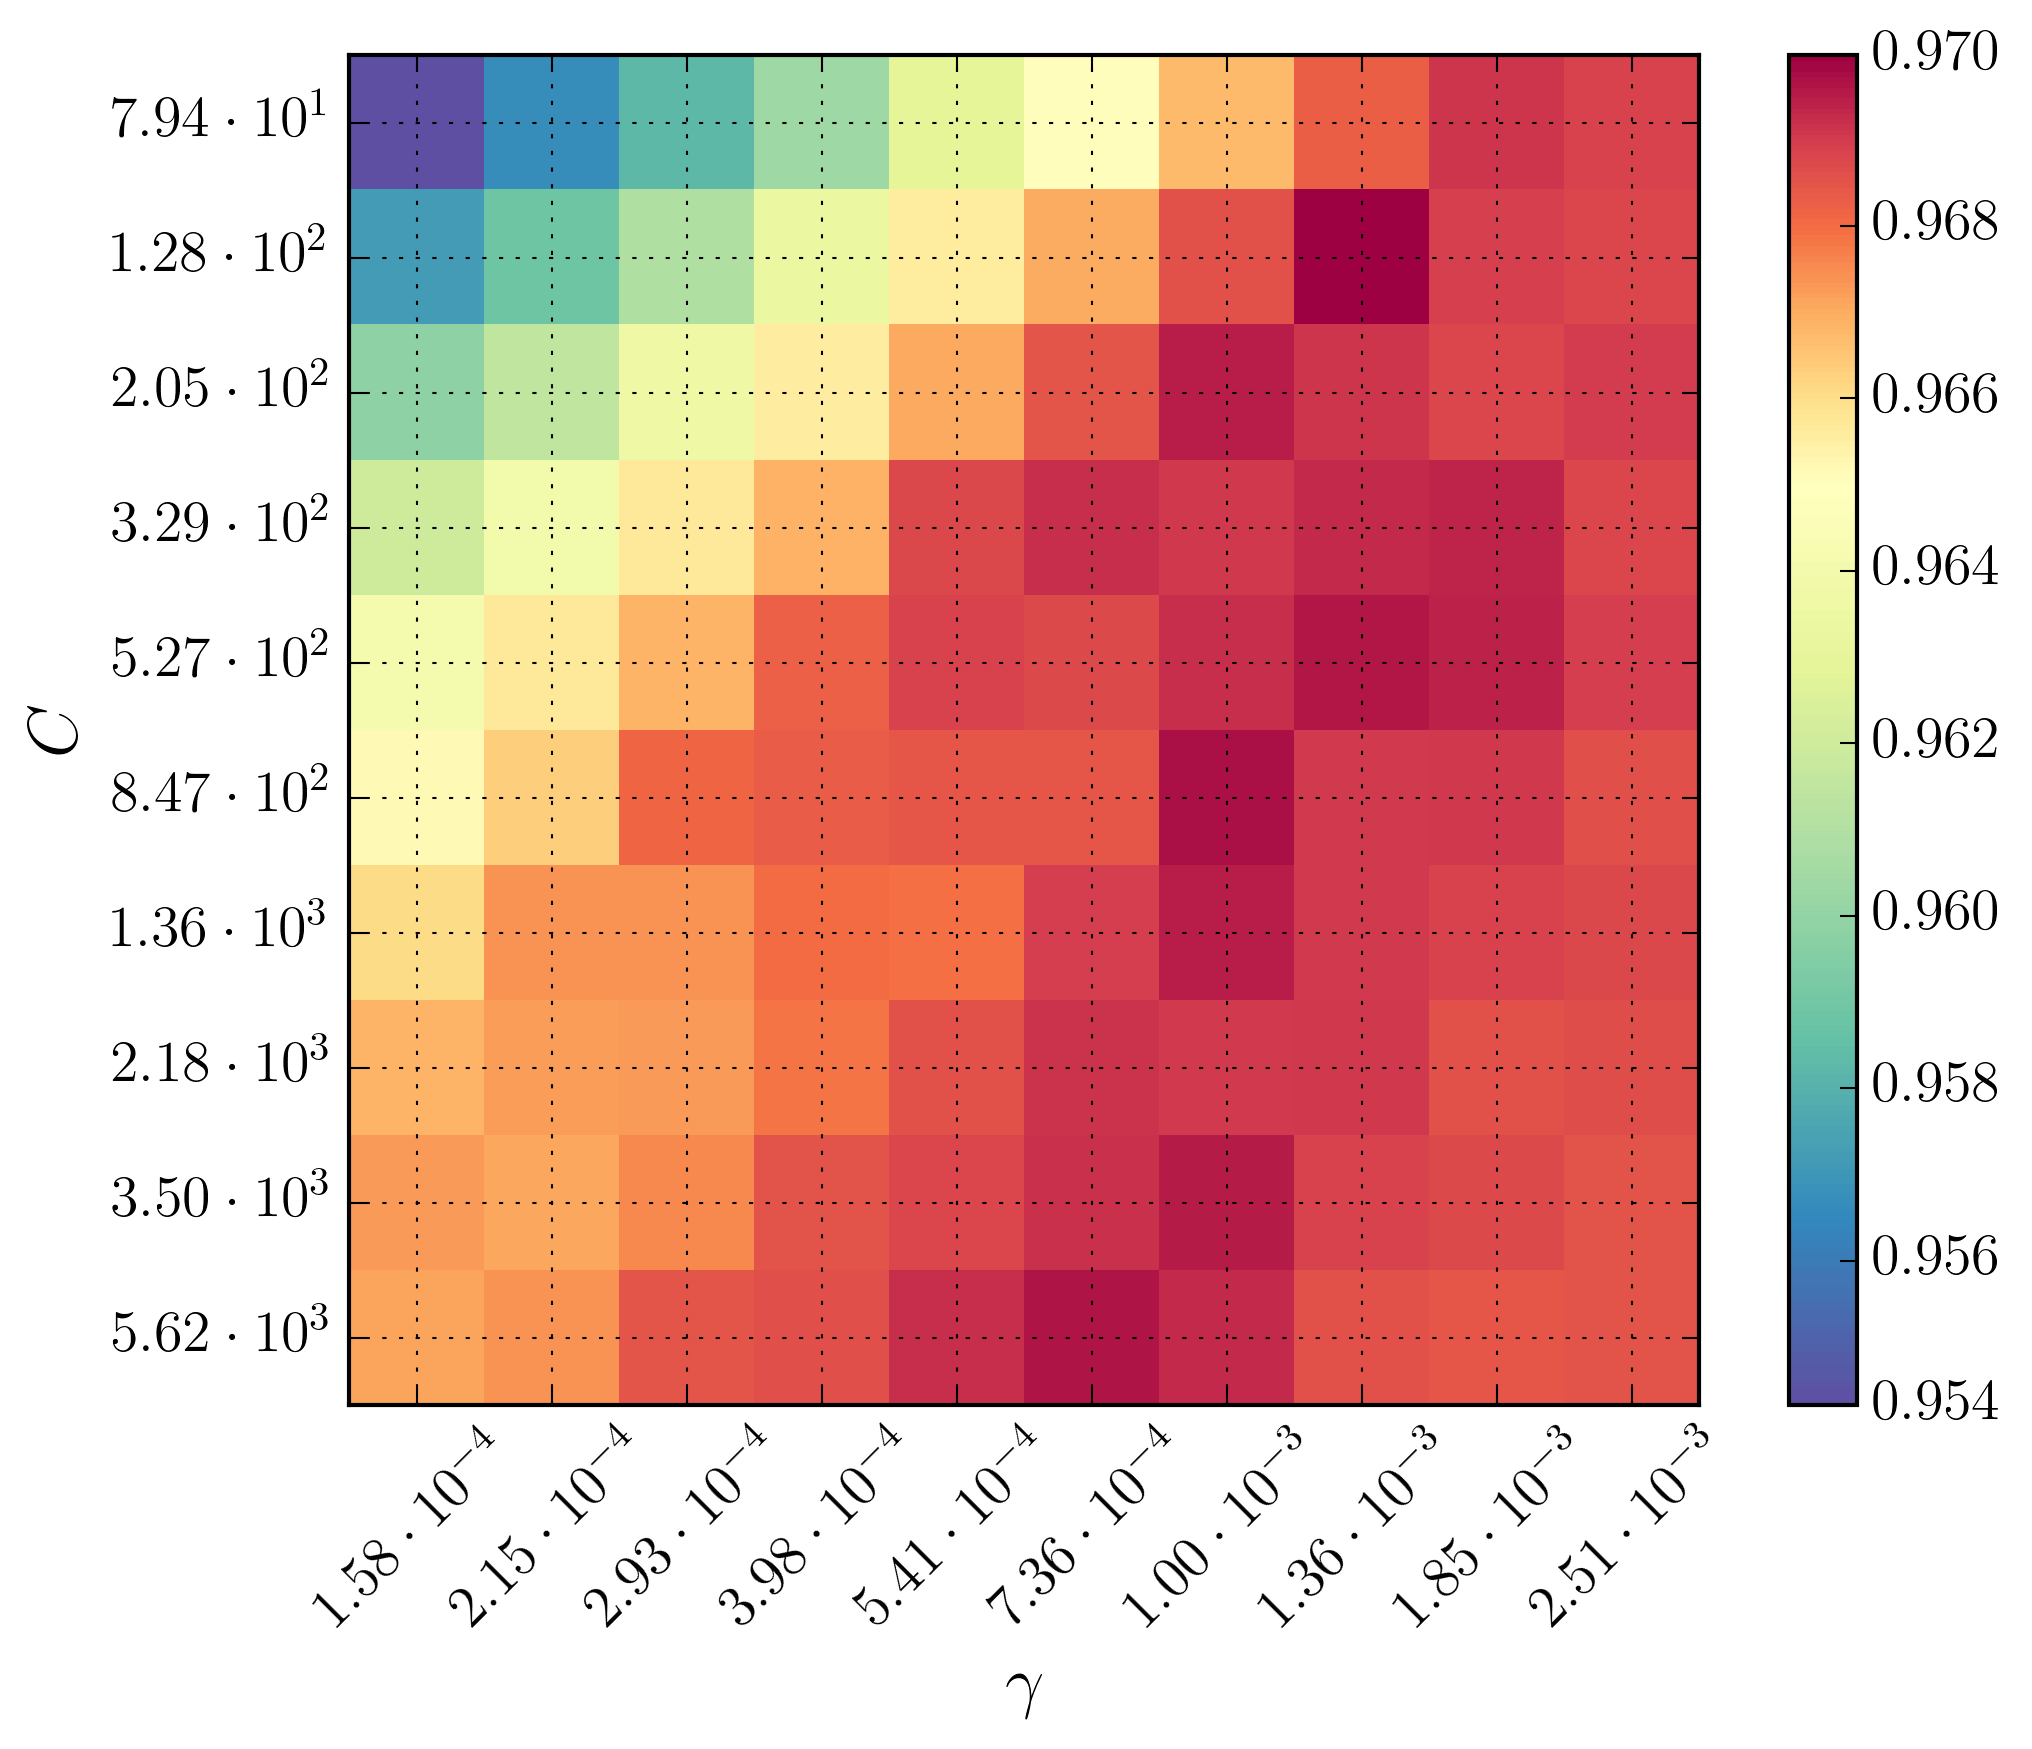
\includegraphics[width=\textwidth]{figures/gridsearch/svm/superclasses/svm-superclasses-04.png}		
	\end{subfigure}
	\begin{subfigure}[t]{0.49\textwidth}
		\centering
		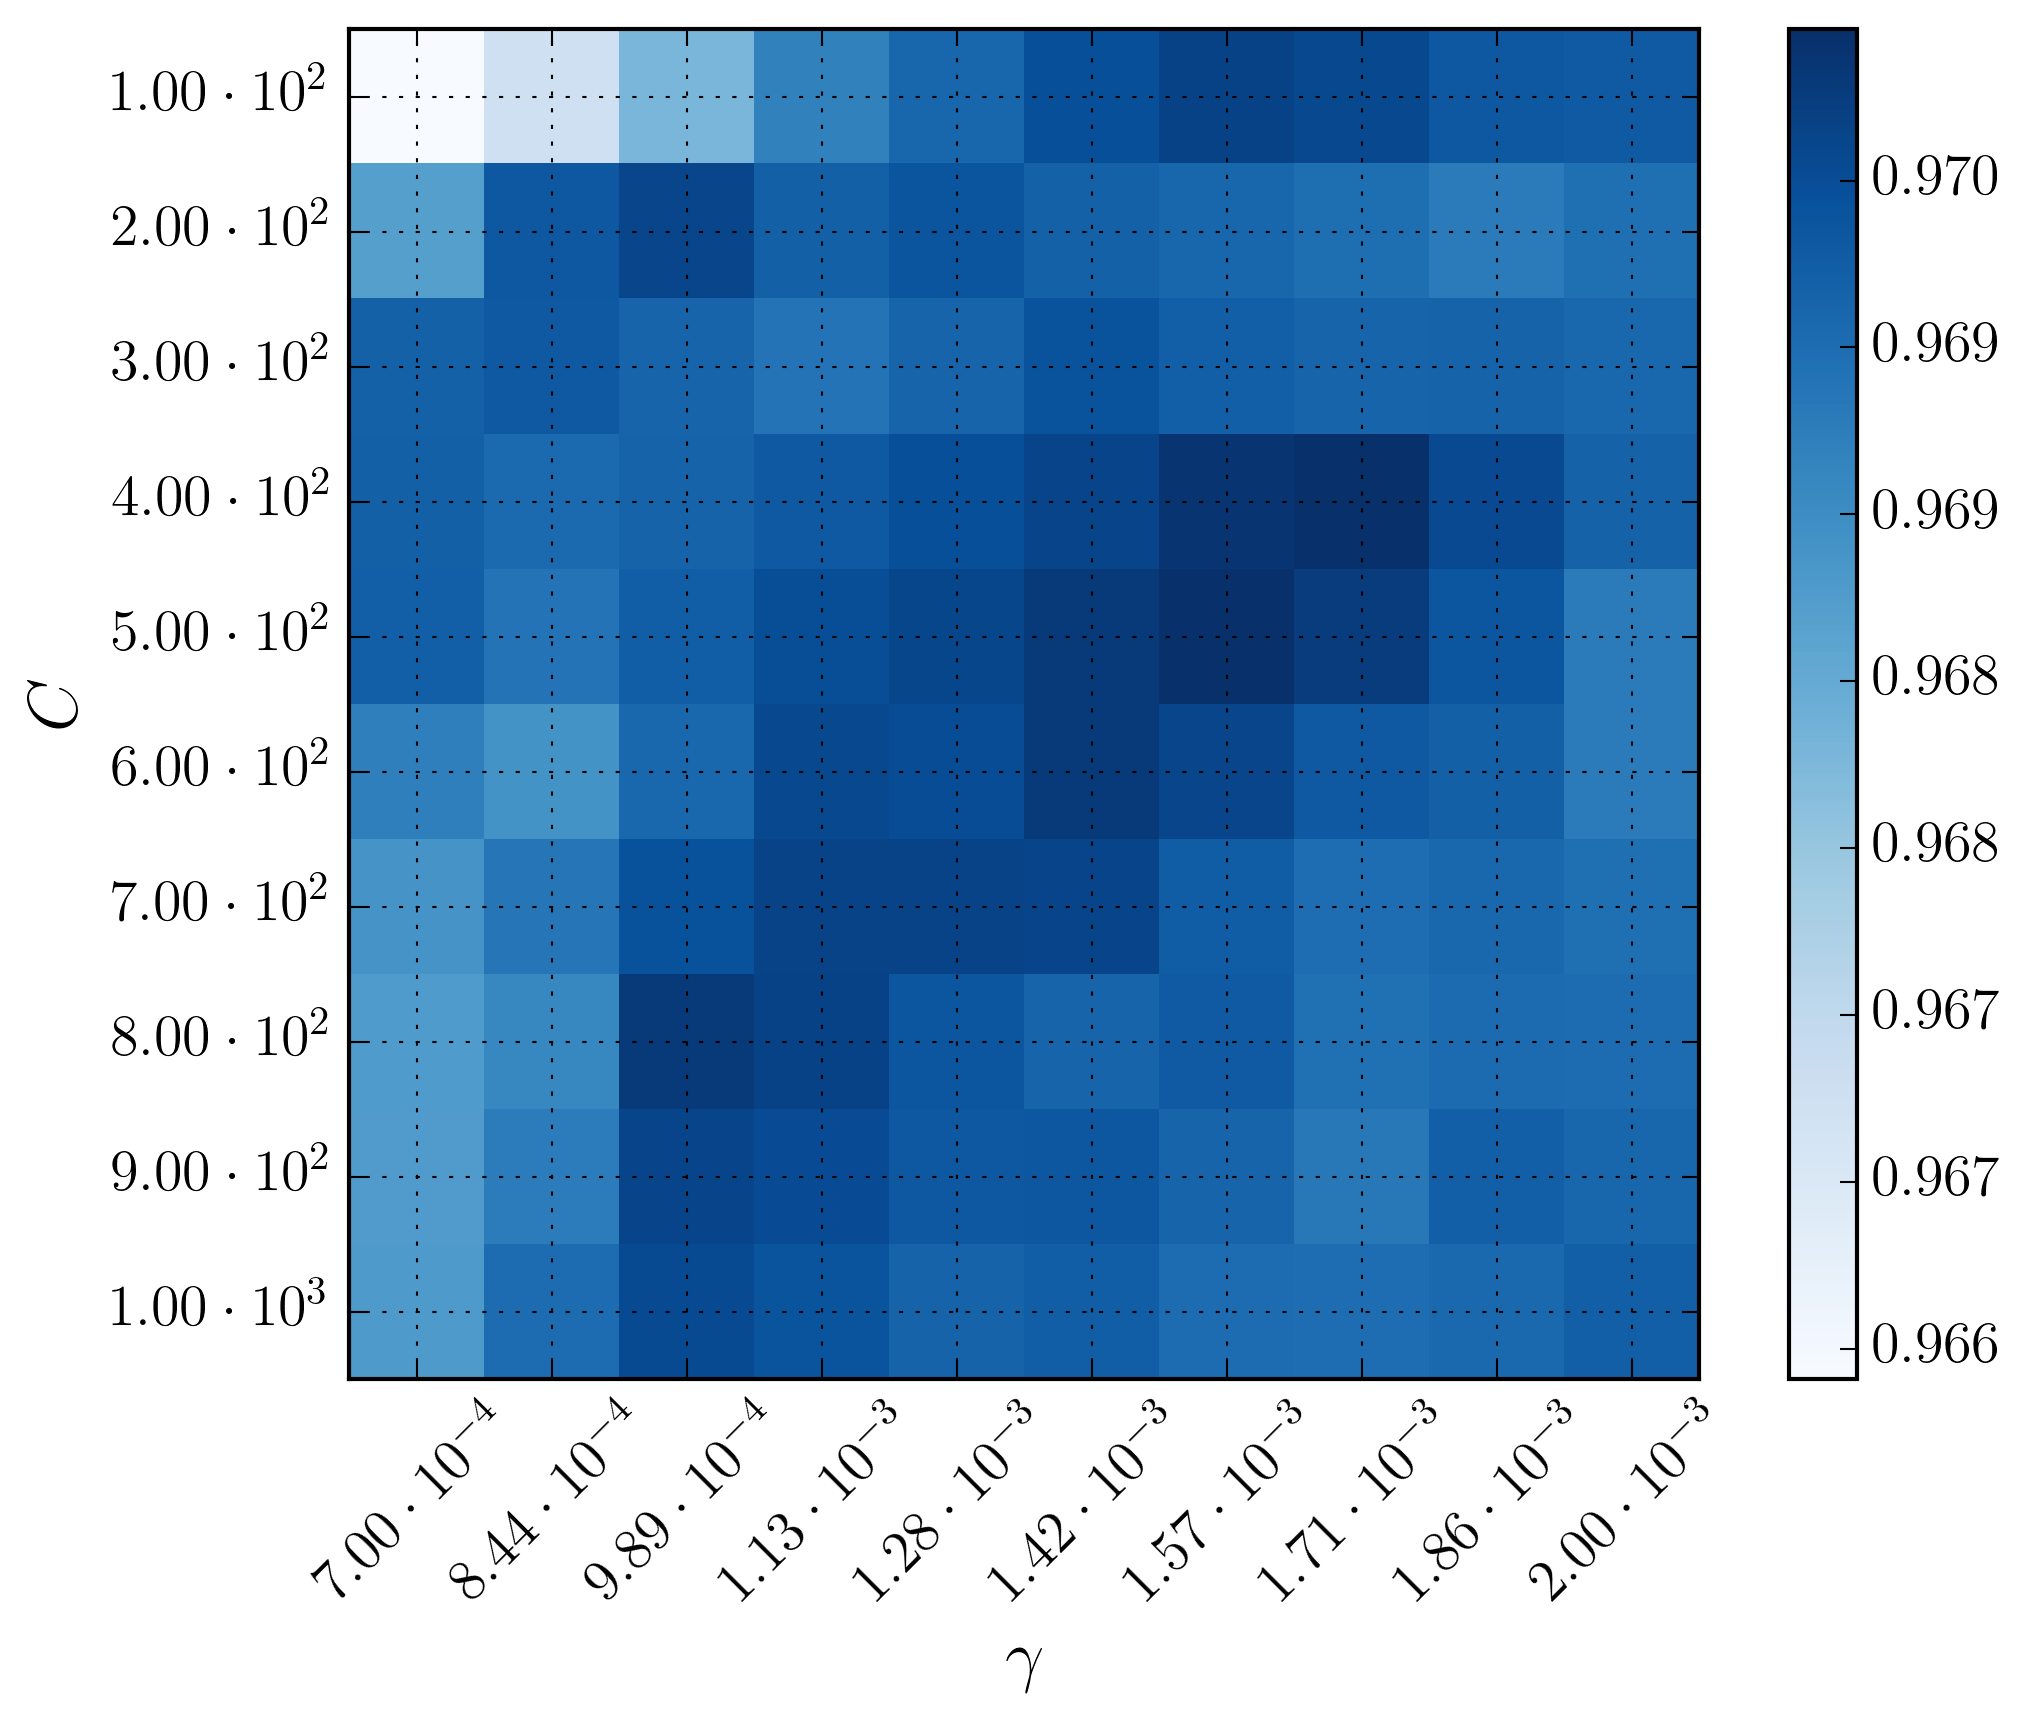
\includegraphics[width=\textwidth]{figures/gridsearch/svm/superclasses/svm-superclasses-05.png}				
	\end{subfigure}
	\begin{subfigure}[t]{0.49\textwidth}
		\centering
		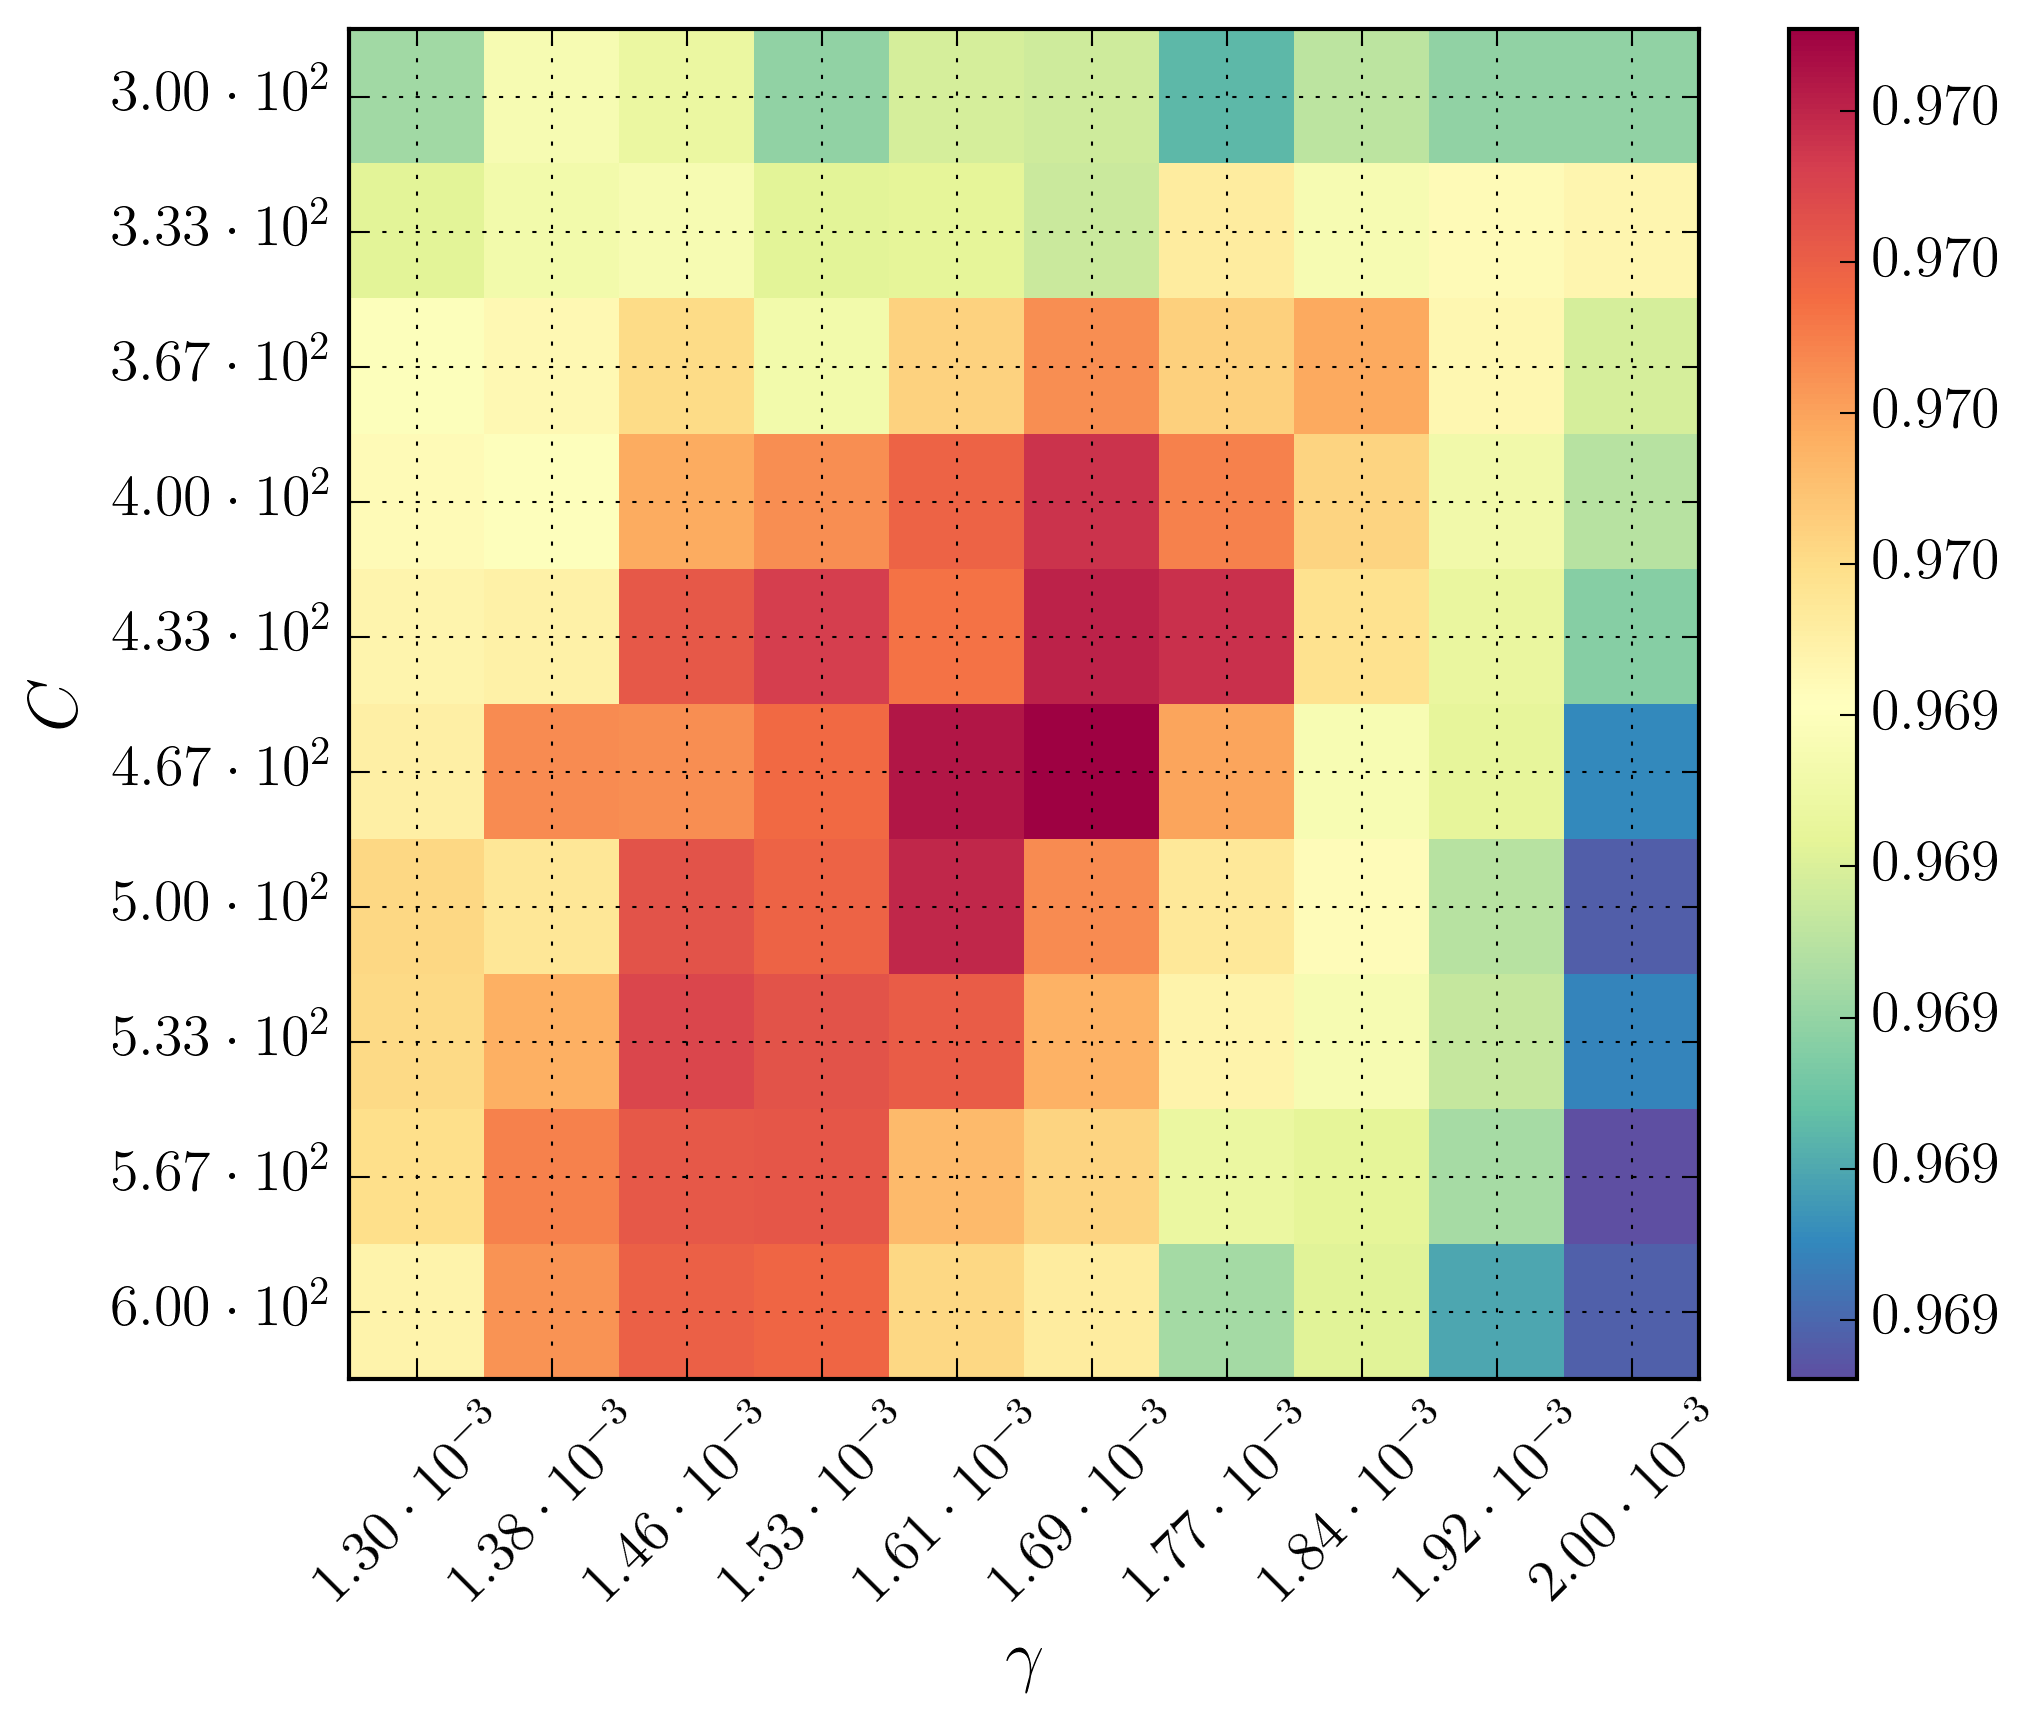
\includegraphics[width=\textwidth]{figures/gridsearch/svm/superclasses/svm-superclasses-06.png}		
	\end{subfigure}
	\caption[Hyperparameter optimization for the Support Vector Machine (SVM)]{This figure shows the average, weighted $F_1$ score on the $C$-$\gamma$-plane during the hyperparameter optimization for the Support Vector Machine. We start looking for global optima on a coarse grid with a wide range (upper left), and adjust the grid toward a finer stepwidth. At some point we find an optimum (lower right)}
	\label{fig:gridsearch-svm-superclasses}
\end{figure}

We determine the optimal hyperparameters for the superclass classification to be $C = 4.67 \cdot 10^{2}$ and $\gamma = 1.69 \cdot 10^{-3}$.

\begin{table}[h]
\centering
\resizebox{\textwidth}{!}{
\begin{tabular}{c|ccccccccc|c}
\toprule
                   & BV        & CEPH       & DSCT      & EB         & LPV         & NoneVar    & QSO       & RRL        & T2CEPH   & $\Sigma $ \\
\midrule
BV                 & {\bfseries 762} &            &           &     12     &     1       &     19     &      1    &            &     1    &     796   \\
CEPH               &     2     & {\bfseries 2218} &           &     13     &     5       &     3      &           &     28     &    12    &    2281   \\
DSCT               &           &      5     & {\bfseries 453} &     8      &             &     17     &           &     28     &          &     511   \\
EB                 &    16     &      16    &     10    & {\bfseries 3336} &     50      &     54     &      5    &     46     &     5    &    3538   \\
LPV                &     5     &      5     &           &     46     & {\bfseries 15884} &     51     &      2    &     2      &          &   15995   \\
NoneVar            &    15     &      1     &     14    &     48     &     65      & {\bfseries 4621} &      24   &     3      &          &    4791   \\
QSO                &     2     &      1     &           &     1      &      1      &     30     & {\bfseries 144} &     1      &          &     180   \\
RRL                &           &      27    &     34    &     60     &      4      &     7      &      0    & {\bfseries 4336} &     2    &    4470   \\
T2CEPH             &     1     &      23    &           &     16     &      6      &     1      &           &     11     & {\bfseries 63} &     121   \\
\bottomrule
Recall ($\%$)      &   95.73   &     97.24  &   88.65   &    94.29   &    99.31    &   96.45    &    80.00  &    97.00   &   52.07  &           \\
\hline
Precision ($\%$)   &   94.89   &     96.60  &   88.65   &    94.24   &    99.18    &   96.21    &    81.82  &    97.33   &   75.90  &           \\
\hline
$F_1$ score ($\%$) &   95.31   &     96.92  &   88.65   &    94.26   &    99.24    &   96.33    &    80.90  &    97.16   &   61.77  & 97.25 $\pm$ 0.25 \\
\bottomrule

\end{tabular}
}
\label{tab:svm-confusion-matrix-superclasses}
\caption{This table shows the confusion matrix for the SVM superclasses classification on the EROS data set with $C = 4.67 \cdot 10^{2}$ and $\gamma = 1.69 \cdot 10^{-3}$. The columns show predicted labels, while rows show the true label.}
\end{table}

Furthermore, we also want the classifier to predict subclasses as well...

\begin{landscape}
\begin{table}[h]
\centering
\resizebox{22cm}{!}{
\begin{tabular}{C{3.1cm}|C{.95cm}C{.95cm}C{.95cm}C{.95cm}C{.95cm}C{.95cm}C{.95cm}C{.95cm}C{.95cm}C{.95cm}C{.95cm}C{.95cm}C{.95cm}C{.95cm}C{.95cm}C{.95cm}C{.95cm}C{.95cm}C{.95cm}C{.95cm}C{.95cm}C{.95cm}C{.95cm}C{.95cm}C{.95cm}|c}
\toprule
 & \rot{BV} &   \rot{1O} &   \rot{F} &   \rot{CEPH Other} &   \rot{DSCT} &    \rot{EC} &    \rot{ED} &   \rot{ED ESD} &   \rot{ESD} &   \rot{EB Other} &   \rot{Mira AGB C} &   \rot{Mira AGB O} &   \rot{OSARG AGB C} &   \rot{OSARG AGB O} &   \rot{OSARG RGB C} &   \rot{OSARG RGB O} &   \rot{SRV AGB C} &   \rot{SRV AGB O} &   \rot{None\-Var} &   \rot{QSO} &   \rot{RRab} &   \rot{RRc} &   \rot{RRd} &   \rot{RRe} &   \rot{T2\-CEPH} &    $\Sigma$ \\
\midrule
BV & \bfseries 766      &     1     &           &              &          &   4      &    2      &             &   2      &     1      &                  &                  &                   &                   &                   &                   &                 &                 &     17      &   2      &            &           &           &           &     1      & 796  \\
1O &   2      &   \bfseries 723     &   51      &      24      &          &   5      &    2      &             &   5      &     2      &                  &                  &            1      &                   &                   &                   &                 &          2      &      2      &          &     9      &   10      &           &           &     6      & 844 \\
F &   1      &    98     & \bfseries 1162      &       4      &          &          &           &             &   1      &            &           1      &                  &                   &                   &                   &                   &                 &          1      &             &          &     3      &           &           &           &     4      & 1275 \\
CEPH Other &          &    34     &    3      &     \bfseries 	114      &          &   2      &           &             &   2      &            &                  &                  &                   &                   &                   &                   &                 &                 &             &          &     2      &    1      &    1      &           &     3      & 162 \\
DSCT &          &     1     &           &              & \bfseries 445      &   2      &    1      &      1      &   7      &     2      &                  &                  &                   &                   &                   &                   &                 &                 &     19      &          &     4      &   11      &    2      &   16      &            & 511 \\
EC &   1      &     8     &    1      &       1      &   4      & \bfseries 272      &    6      &      1      &  88      &    16      &                  &                  &            2      &                   &                   &           11      &                 &          1      &      4      &   1      &    13      &    3      &    2      &    5      &     5      & 445 \\
ED &   6      &     1     &           &       1      &   3      &  17      & \bfseries 1246      &     91      & 234      &    17      &                  &                  &            1      &            1      &                   &            1      &                 &                 &     24      &   1      &            &           &           &           &            & 1644 \\
ED ESD &          &           &           &              &   3      &   1      &   85      &    \bfseries 15      &  24      &     2      &                  &                  &                   &                   &                   &                   &                 &          1      &     14      &          &     1      &           &           &           &            & 146 \\
ESD &   9      &     4     &    1      &       1      &   2      & 140      &  204      &     35      & \bfseries 694      &    27      &                  &                  &                   &            3      &                   &           11      &                 &                 &      8      &          &     3      &    6      &           &    2      &            & 1150 \\
EB Other &   2      &     2     &           &              &   1      &  25      &   22      &      2      &  47      &    \bfseries 18      &                  &                  &            3      &            5      &                   &           10      &                 &                 &      9      &   2      &     3      &    1      &           &    1      &            & 153 \\
Mira AGB C &   1      &           &           &              &          &   1      &           &             &          &            &         \bfseries 689      &          15      &                   &                   &                   &            1      &         39      &          2      &      5      &   1      &            &           &           &           &            & 754 \\
Mira AGB O &          &           &           &              &          &          &           &             &          &            &          23      &        \bfseries 271      &                   &                   &                   &                   &          2      &         32      &      1      &          &            &           &           &           &            & 329 \\
OSARG	AGB C &   1      &           &           &              &          &          &           &             &          &            &           1      &                  &          \bfseries 958      &          206      &            5      &           13      &        198      &         15      &     19      &          &            &           &           &           &            & 1416 \\
OSARG AGB O &          &           &           &              &          &          &           &             &   1      &     4      &                  &                  &          388      &         \bfseries 2360      &            1      &          192      &         18      &        379      &     24      &          &     1      &           &           &           &            & 3368 \\
OSARG RGB C &          &           &           &              &          &          &           &             &          &            &           1      &                  &            8      &           11      &            \bfseries 6      &           20      &          6      &          2      &      2      &          &     1      &           &           &           &            & 57 \\
OSARG RGB O &   2      &           &    1      &              &          &  13      &    2      &             &   9      &     4      &           1      &                  &           22      &          149      &           21      &         \bfseries 1729      &          1      &         86      &      6      &          &            &           &           &           &            & 2046 \\
SRV AGB C &   1      &           &           &              &          &          &           &             &          &            &          93      &           2      &          301      &           18      &            3      &            4      &       \bfseries 3315      &         74      &      8      &          &            &           &           &           &            & 3819  \\
SRV AGB O &          &     1     &           &              &          &          &           &             &          &            &           7      &          72      &           58      &          329      &           15      &          136      &        106      &       \bfseries 3479      &      3      &          &            &           &           &           &            & 4206 \\
NoneVar &  16      &           &           &              &  13      &   1      &   21      &      4      &  12      &     6      &           2      &                  &           20      &           34      &            4      &           14      &          1      &                 &   \bfseries 4613      &  28      &            &    1      &    1      &           &            & 4791 \\
QSO &   2      &           &           &              &          &   1      &           &             &   1      &            &           1      &                  &                   &                   &                   &                   &                 &                 &     33      & \bfseries 142      &            &           &           &           &            & 180 \\
RRab &          &    11     &    9      &       1      &   1      &  28      &           &             &  12      &     2      &                  &                  &                   &                   &            1      &                   &                 &                 &      9      &   1      &  \bfseries 3248      &   62      &   42      &    5      &     2      & 3434 \\
RRc &          &     5     &           &       2      &  11      &   5      &    3      &      1      &   6      &     4      &                  &                  &                   &                   &                   &                   &                 &                 &      2      &          &    46      &  \bfseries 574      &   23      &   32      &            & 714 \\
RRd &          &           &           &       1      &   1      &   4      &           &             &          &            &                  &                  &                   &                   &                   &                   &                 &                 &      1      &          &    42      &   40      &   \bfseries 89      &    1      &            & 179 \\
RRe &          &     1     &           &              &  22      &   4      &    1      &      1      &   4      &     1      &                  &                  &                   &                   &            1      &                   &                 &                 &             &          &     4      &   57      &    1      &   \bfseries 46      &            & 143 \\
T2CEPH &   1      &    16     &    4      &       5      &          &   8      &           &             &   5      &     3      &           2      &                  &                   &                   &                   &                   &          1      &          3      &      2      &          &    10      &           &           &           &    \bfseries 61      & 121 \\
\hline
Recall ($\%$) &   96.23 &    85.66 &   91.14 &       70.37 &   87.08 &   61.12 &   75.79 &      10.27 &    60.35 &     11.76 &           91.38 &           82.37 &            67.66 &            70.07 &            10.53 &             84.51 &          86.80 &          82.72 &      96.28 &  78.89 &     94.58 &    80.39 &    49.72 &    32.17 &     50.41 &        \\[.1cm]
\hline
Precision ($\%$) &      94.45 &     79.80 &    94.32 &       74.03 &   87.94 &   51.03 &    78.12 &      9.93 &   60.14 &     16.51 &           83.92 &           75.28 &            54.37 &            75.74 &            10.53 &            80.72 &          89.91 &          85.33 &      95.61 &   79.78 &     95.81 &    74.93 &    55.28 &    42.59 &     74.39 &        \\[.1cm]
\hline
$F_1$-score ($\%$) &   95.33 &    82.63 &   92.70 &       72.15 &   87.51 &   55.62 &   76.94 &      10.10 &    60.24 &     13.74 &           87.49 &           78.67 &            60.29 &            72.79 &           10.53 &             82.57 &          88.33 &          84.00 &      95.94 &  79.33 &     95.19 &   77.56  &  52.35   &  36.65   &     60.10 & $82.75 \pm 0.47$        \\[.1cm]
\bottomrule
\end{tabular}
}
\label{tab:svm-confusion-matrix-subclasses}
\caption{This table shows the confusion matrix for the SVM subclasses classification on the EROS data set with $C = 9.83 \cdot 10^{2}$ and $\gamma = 9.22 \cdot 10^{-4}$. The columns show predicted labels, while rows show the true label.}

\end{table}
\end{landscape}
\section{Performance of the Random Forest Classifier}

The second classifier to evaluate is the Random Forest classifier. Once again, for optimal classification performance, we have to optimize the model's hyperparameters $t$, the number of trees in the forest, and $m$, the maximum number of features to consider at each split. The results of the $5$-fold cross--validation grid search (superclasses), optimized for the average $F_1$-score, weighted by the number of observations per class, shown in figure \ref{fig:gridsearch-rf-superclasses}.

\begin{figure}[h]
	\centering
	\begin{subfigure}[t]{0.49\textwidth}
		\centering
		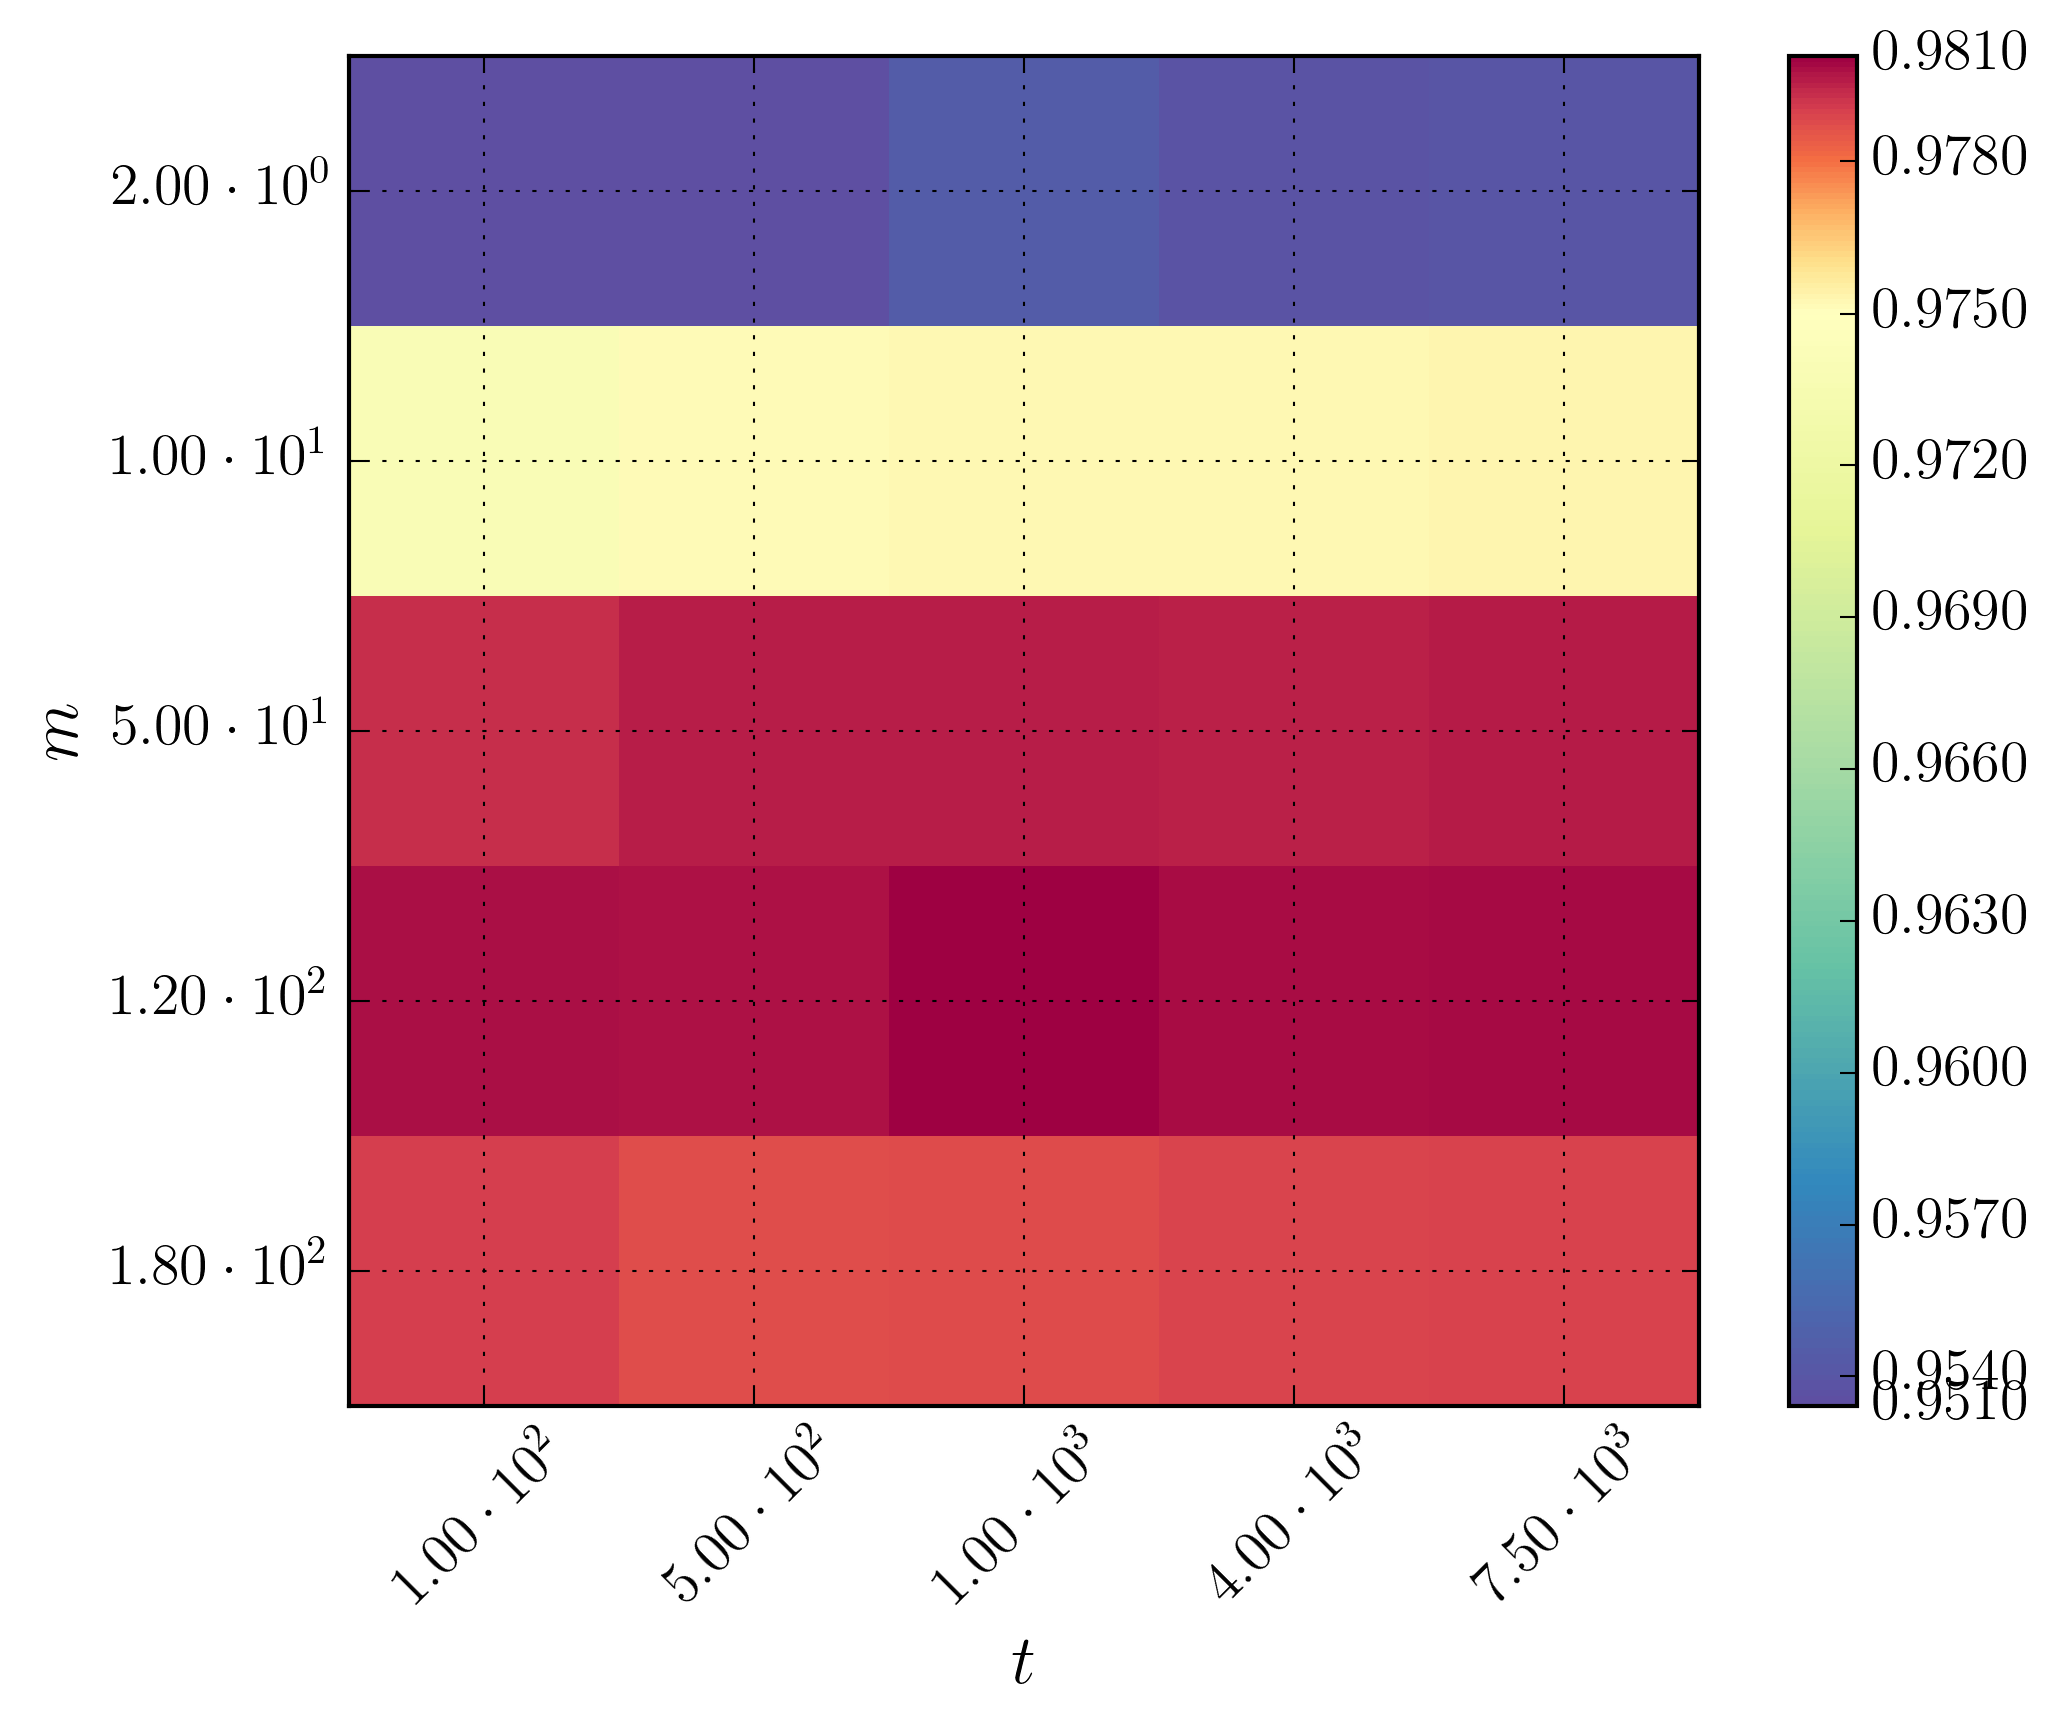
\includegraphics[width=\textwidth]{figures/gridsearch/rf/superclasses/rf-superclasses-01.png}				
	\end{subfigure}
	\begin{subfigure}[t]{0.49\textwidth}
		\centering
		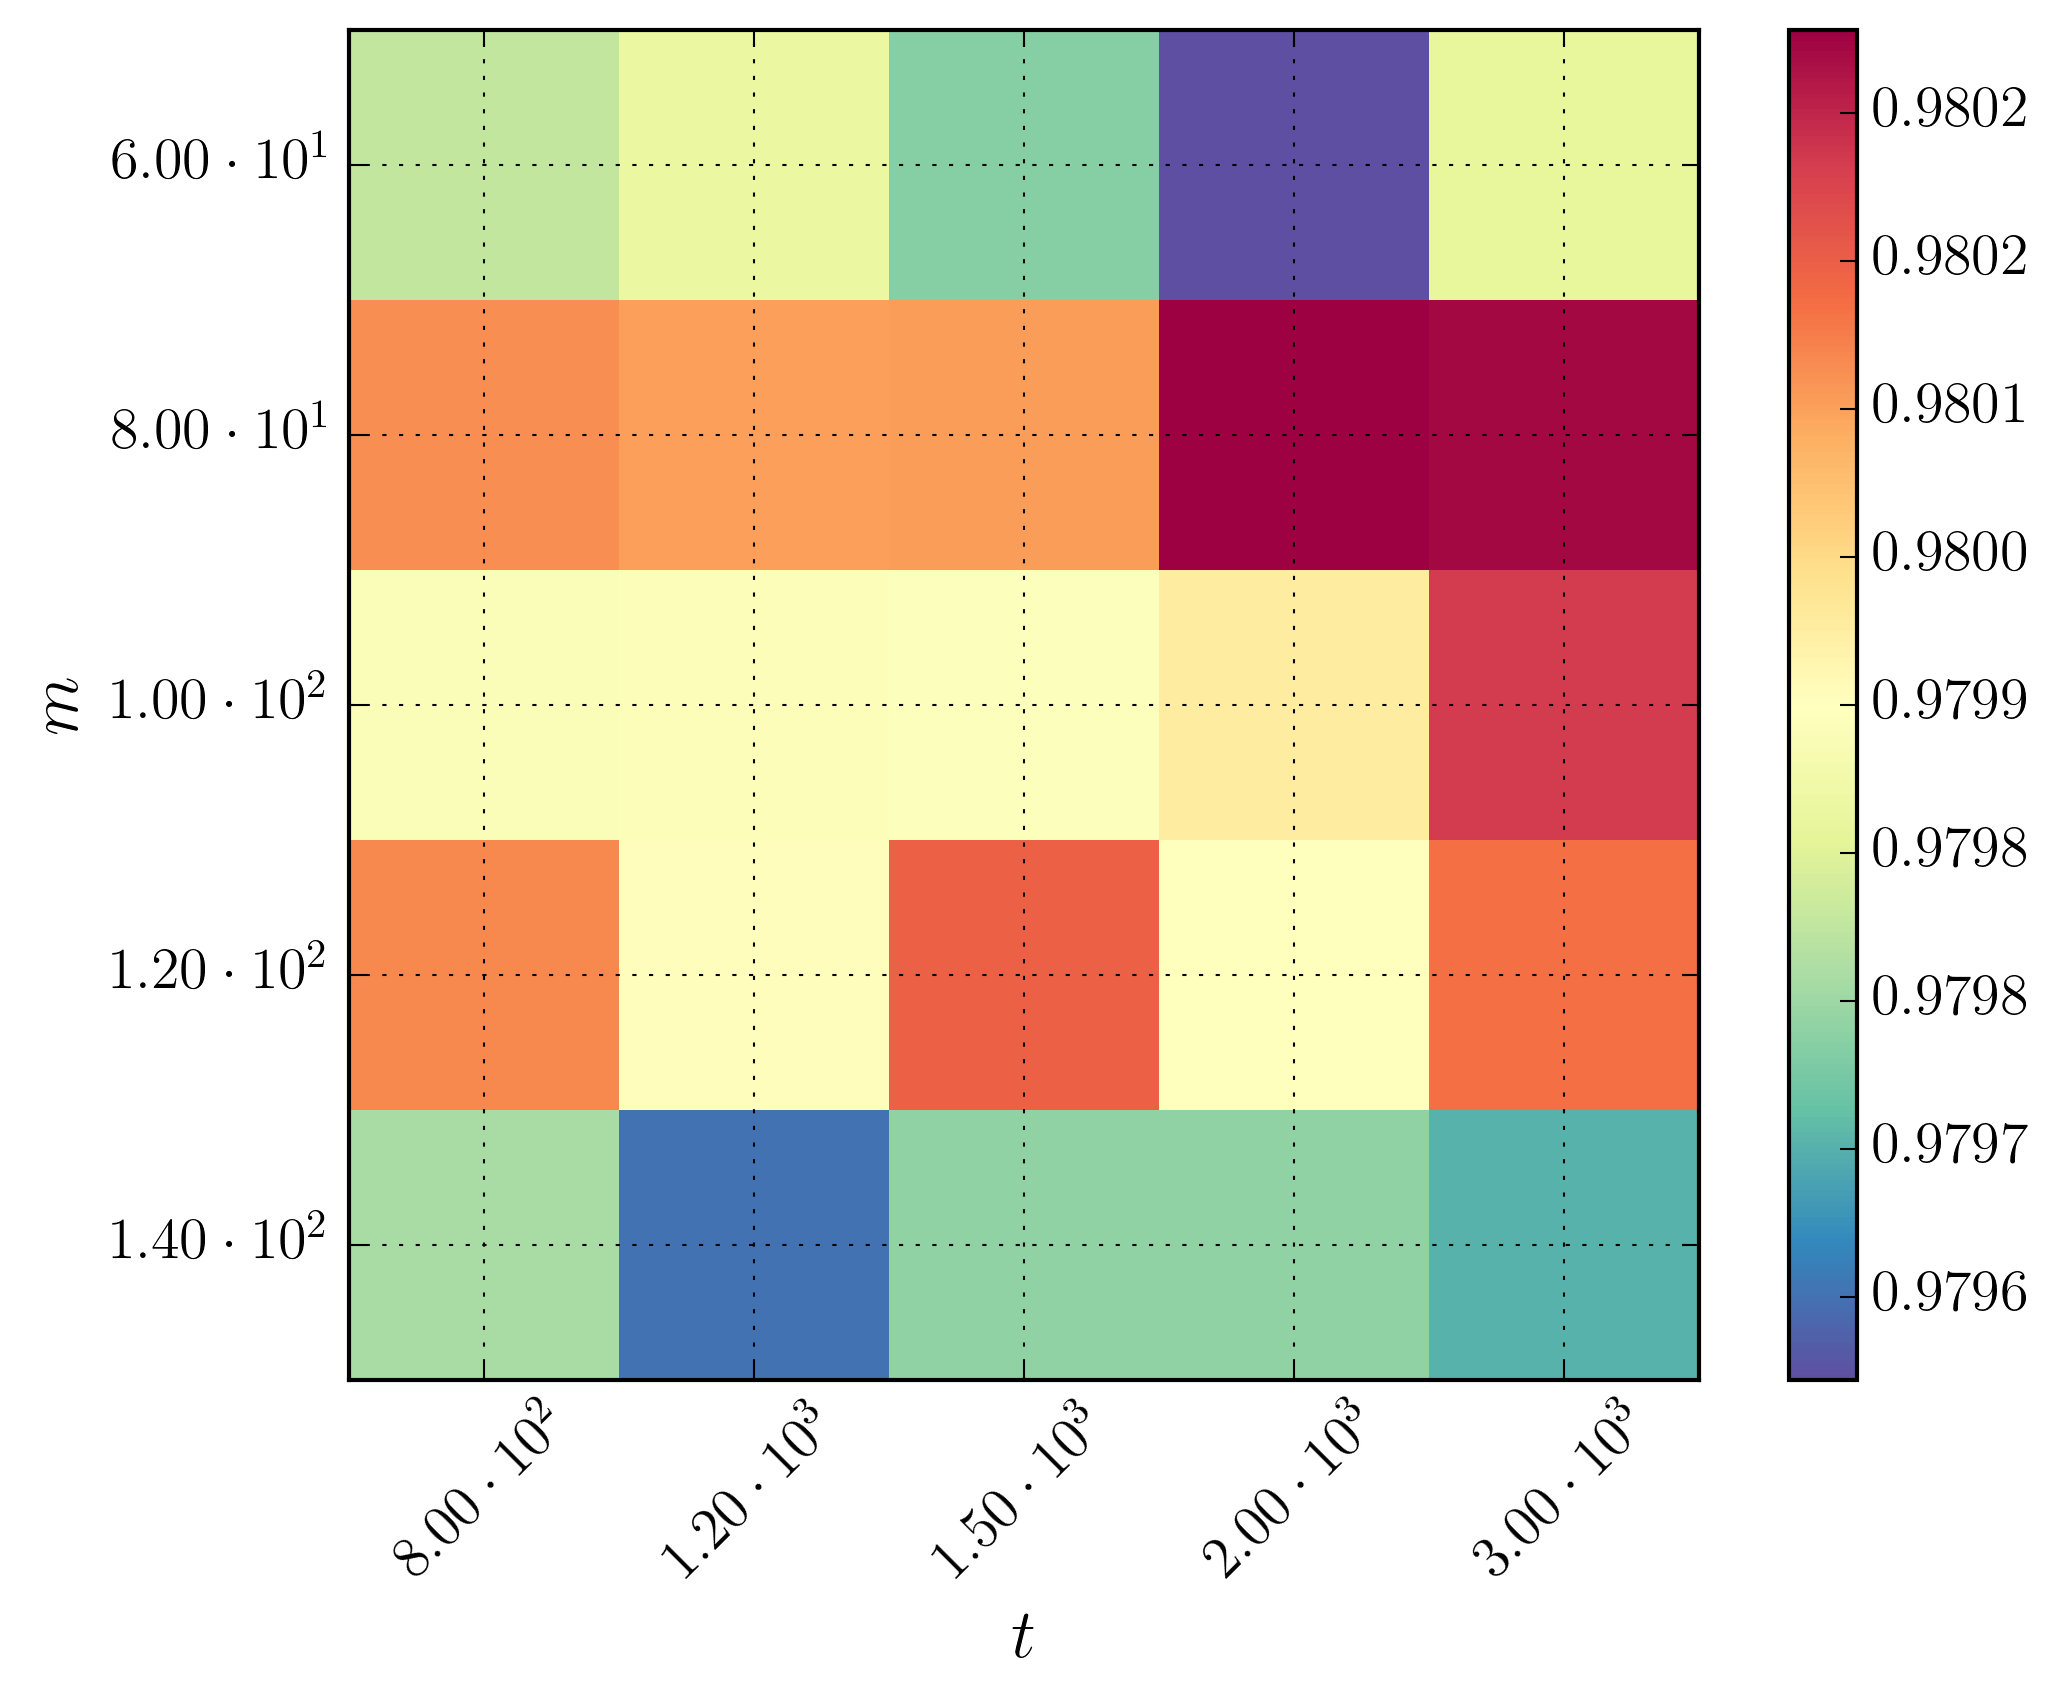
\includegraphics[width=\textwidth]{figures/gridsearch/rf/superclasses/rf-superclasses-02.png}		
	\end{subfigure}
	\begin{subfigure}[t]{0.49\textwidth}
		\centering
		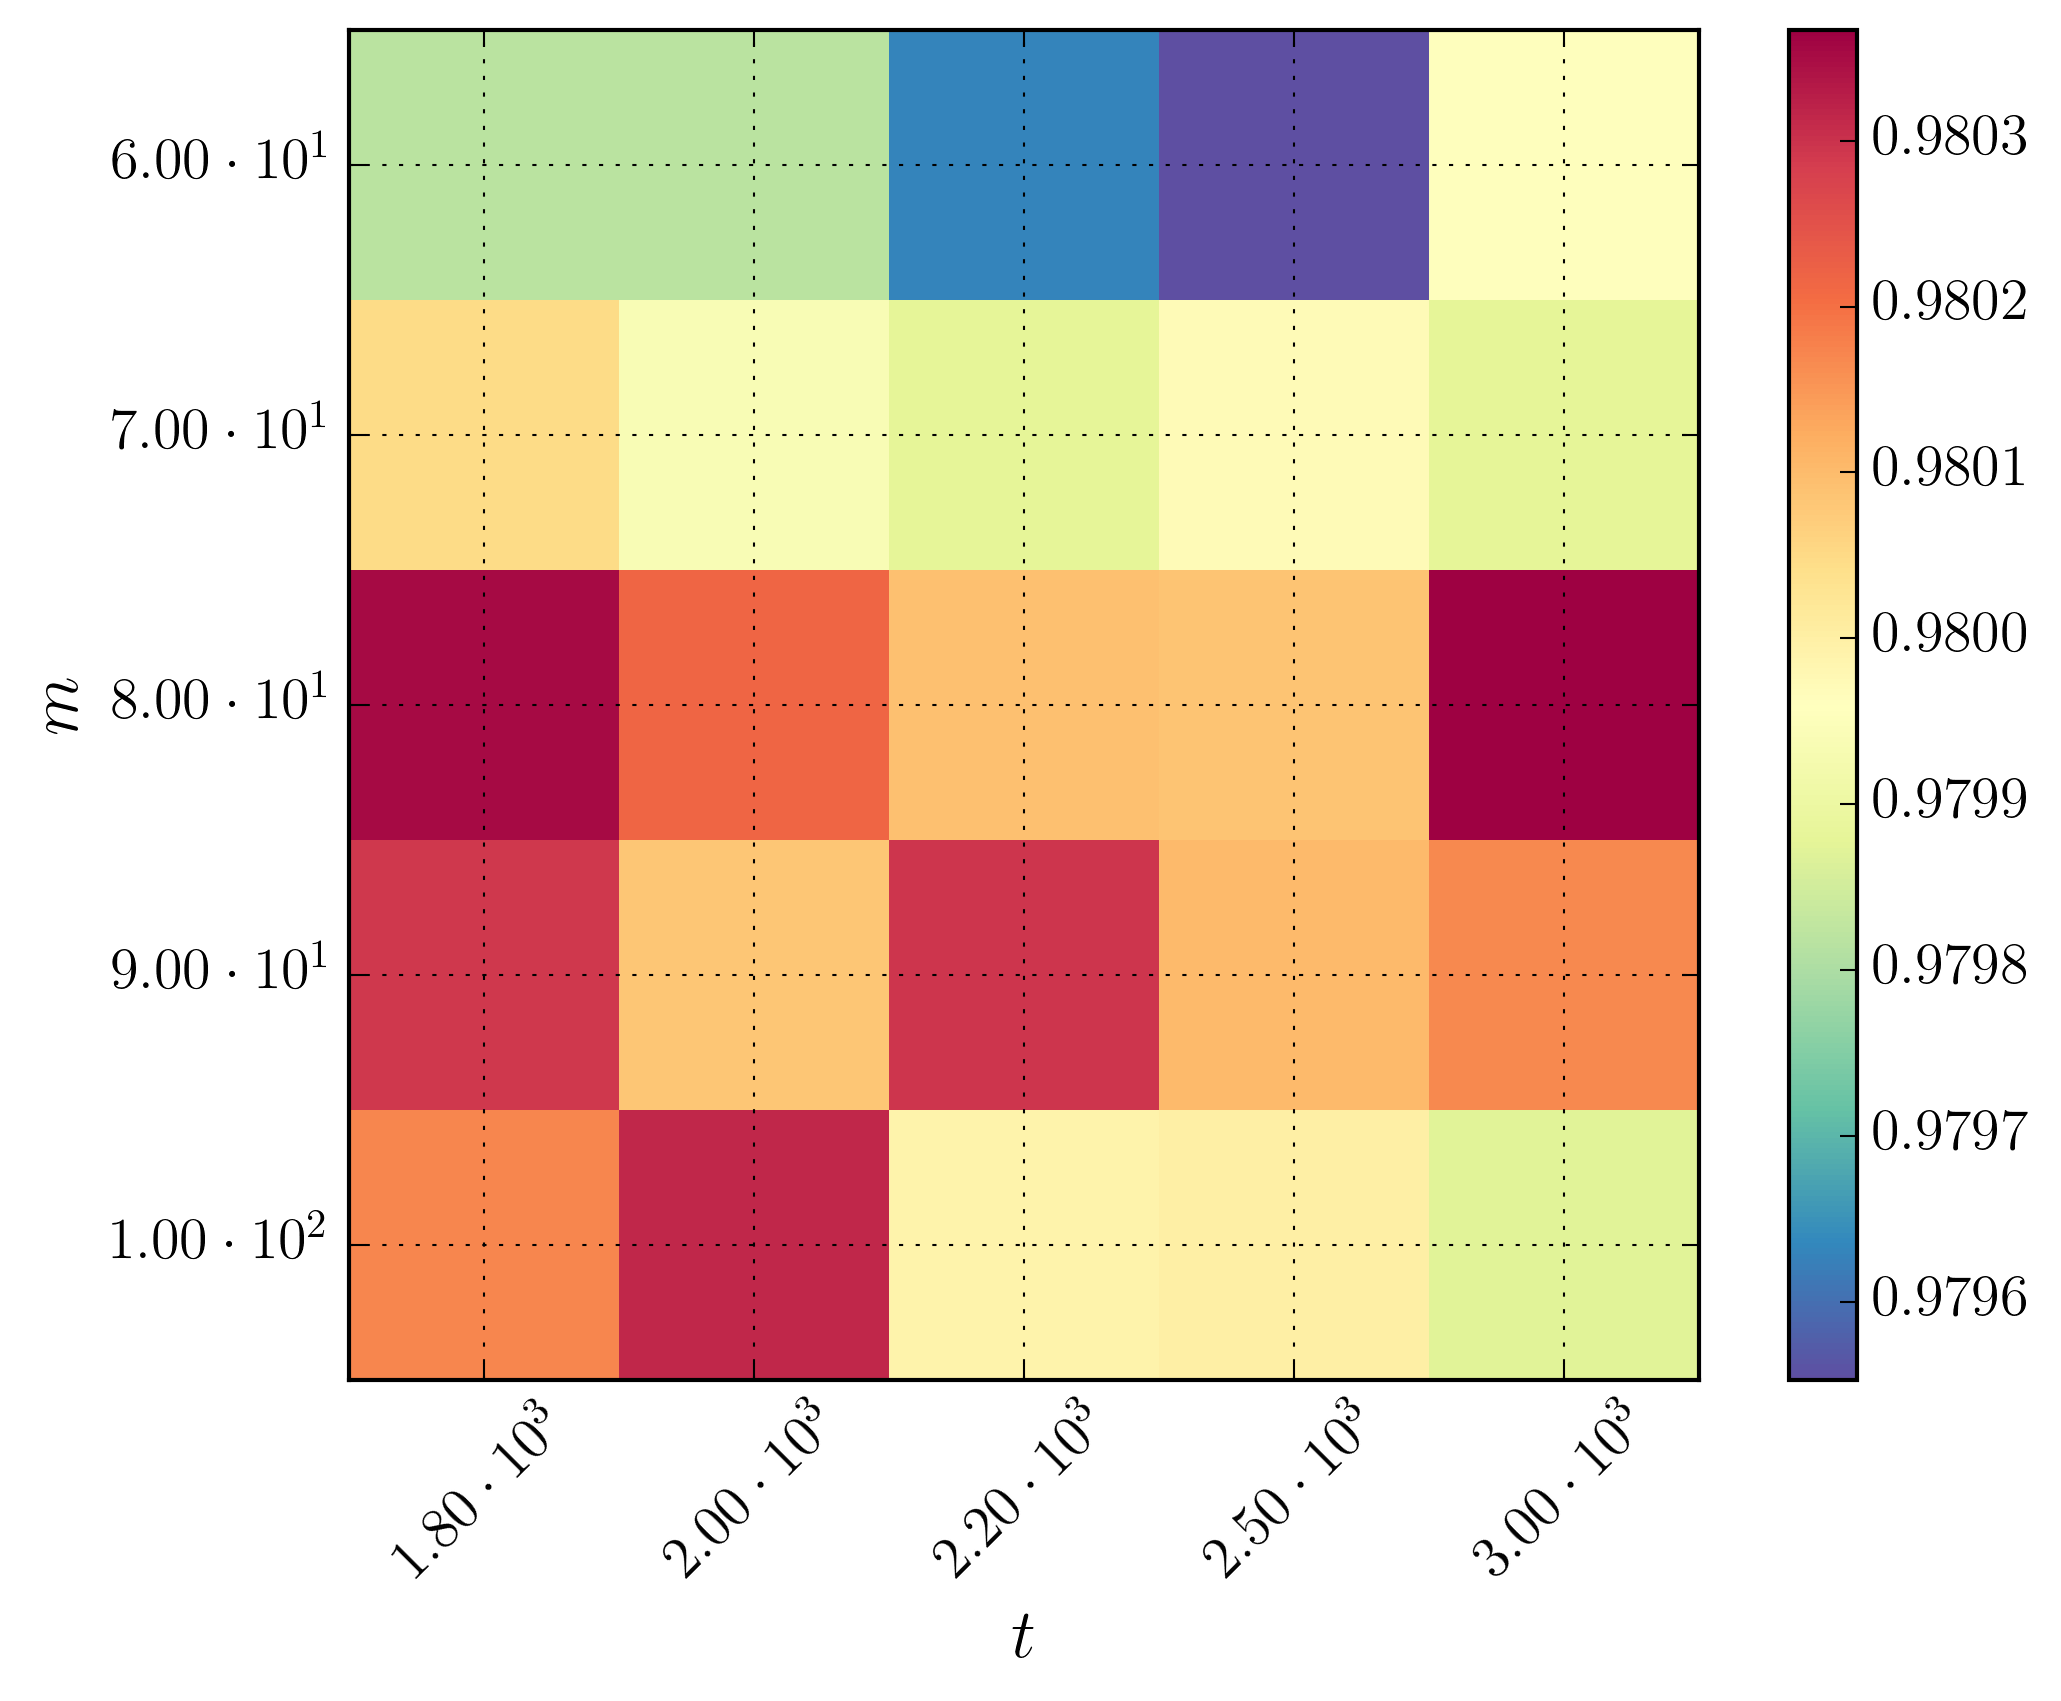
\includegraphics[width=\textwidth]{figures/gridsearch/rf/superclasses/rf-superclasses-03.png}				
	\end{subfigure}
	\begin{subfigure}[t]{0.49\textwidth}
		\centering
		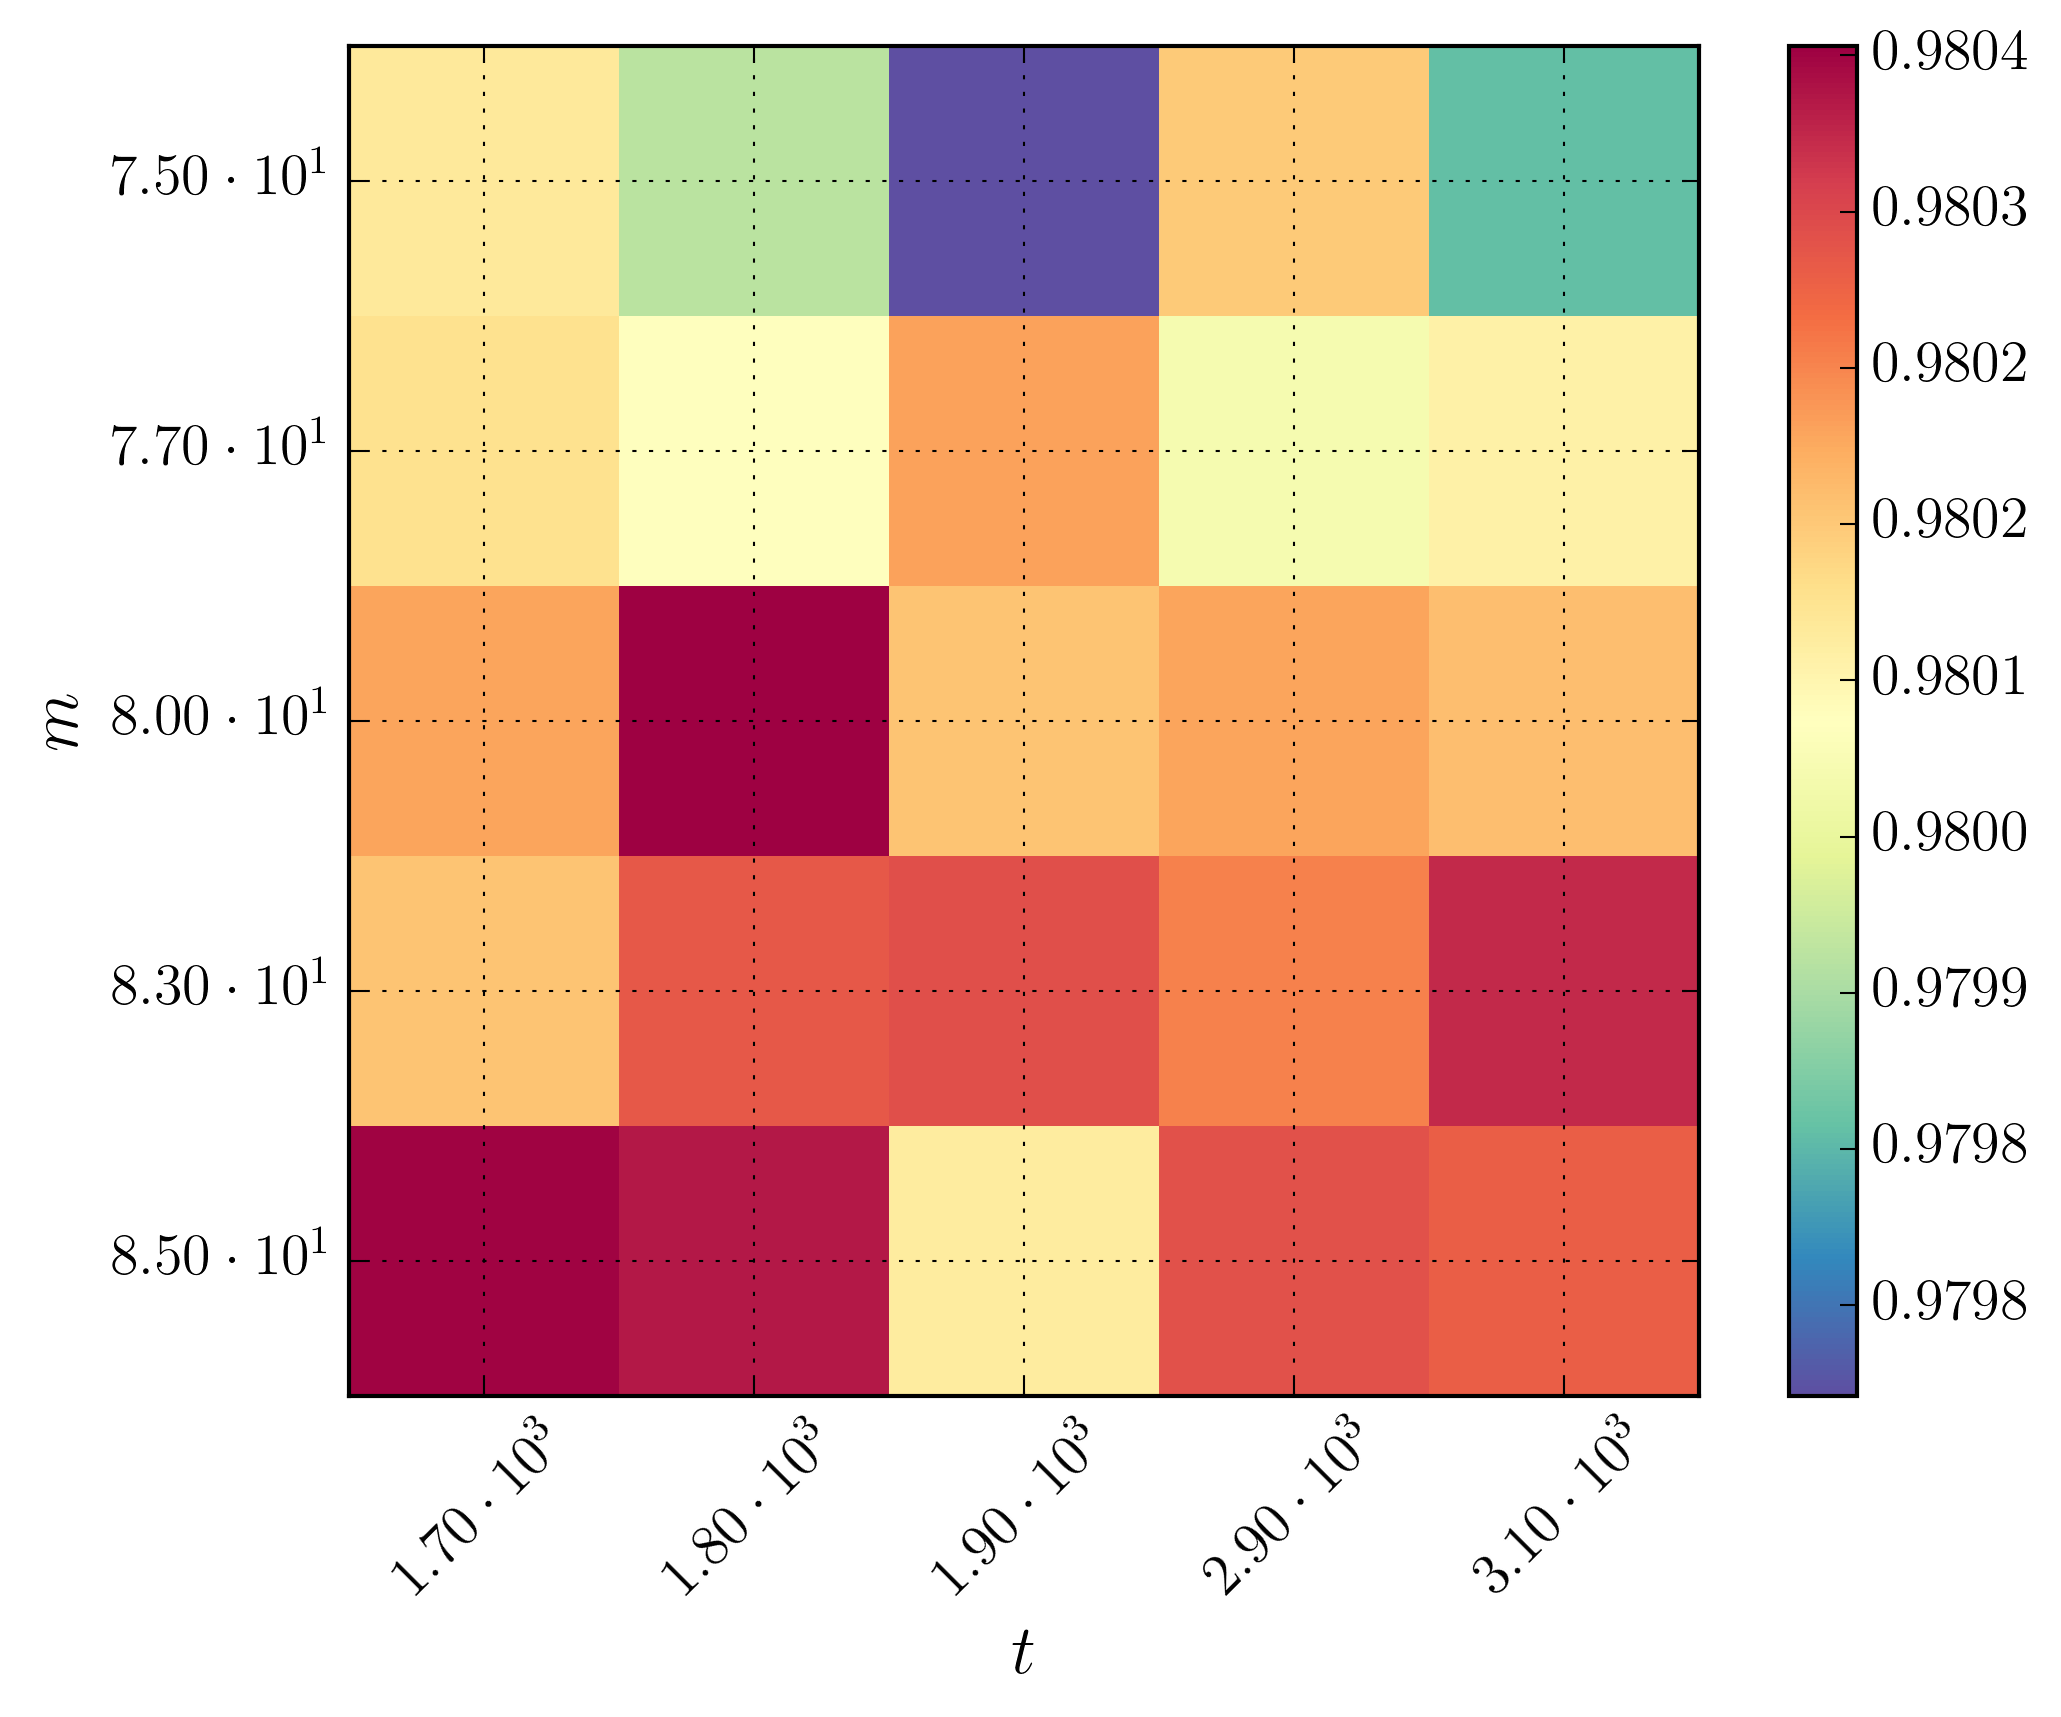
\includegraphics[width=\textwidth]{figures/gridsearch/rf/superclasses/rf-superclasses-04.png}		
	\end{subfigure}		
	\caption[Hyperparameter optimization for the Random Forest Classifier]{This figure shows the average, weighted $F_1$ score on the $m$-$t$-plane during the hyperparameter optimization for the Random Forest Classifier, where $t$ is the number of trees in the forest, and $m$ denotes the maximum number of features considered at each split.}
	\label{fig:gridsearch-rf-superclasses}
\end{figure}

\begin{table}[h]
\centering
\resizebox{\textwidth}{!}{
\begin{tabular}{c|ccccccccc|c}
\toprule
                   & BV        & CEPH       & DSCT      & EB         & LPV         & NoneVar    & QSO       & RRL        & T2CEPH   & $\Sigma $ \\
\midrule
BV                 & {\bfseries 773} &            &           &     11     &      3      &      8     &      1    &            &          &     796   \\
CEPH               &     1     & {\bfseries 2226} &           &     18     &      2      &      3     &           &     31     &          &    2281   \\
DSCT               &           &            & {\bfseries 496} &      2     &             &     12     &           &      1     &          &     511   \\
EB                 &     7     &      7     &     2     & {\bfseries 3342} &     52      &     79     &      3    &     43     &     3    &    3538   \\
LPV                &     4     &      2     &           &     10     & {\bfseries 15945} &     32     &      1    &     1      &          &   15995   \\
NoneVar            &    23     &      1     &     4     &     35     &     72      & {\bfseries 4648} &      8    &            &          &    4791   \\
QSO                &           &            &           &      3     &      4      &     25     & {\bfseries 147} &     1      &          &     180   \\
RRL                &           &      9     &     7     &     31     &      2      &     7      &           & {\bfseries 4414} &          &    4470   \\
T2CEPH             &     1     &      15    &           &     19     &      5      &     3      &           &            & {\bfseries 78} &     121   \\
\bottomrule
Recall ($\%$)      &   97.11   &     97.59  &   97.06   &    94.46   &    99.69    &   97.02    &   81.67   &    98.75   &   64.46  &           \\
\hline
Precision ($\%$)   &   95.55   &     98.50  &   97.45   &    96.28   &    99.13    &   96.49    &   91.87   &    98.29   &   96.93  &           \\
\hline
$F_1$ score ($\%$) &   96.32   &     98.04  &   97.25   &    95.36   &    99.41    &   96.75    &   86.47   &    98.52   &   77.43  & 98.14 $\pm$ 0.07 \\
\bottomrule
\end{tabular}
}
\label{tab:rf-confusion-matrix-superclasses}
\caption{This table shows the confusion matrix for the Random Forest superclasses classification on the EROS data set with $m = 80$ and $t = 1800$. The columns show predicted labels, while rows show the true label.}
\end{table}

\chapter{Assessing Classification Performance for GAIA}

% Simulating GAIA time series
% Performance of the best classifier on GAIA data